\documentclass[twoside]{book}

% Packages required by doxygen
\usepackage{fixltx2e}
\usepackage{calc}
\usepackage{doxygen}
\usepackage[export]{adjustbox} % also loads graphicx
\usepackage{graphicx}
\usepackage[utf8]{inputenc}
\usepackage{makeidx}
\usepackage{multicol}
\usepackage{multirow}
\PassOptionsToPackage{warn}{textcomp}
\usepackage{textcomp}
\usepackage[nointegrals]{wasysym}
\usepackage[table]{xcolor}

% Font selection
\usepackage[T1]{fontenc}
\usepackage[scaled=.90]{helvet}
\usepackage{courier}
\usepackage{amssymb}
\usepackage{sectsty}
\renewcommand{\familydefault}{\sfdefault}
\allsectionsfont{%
  \fontseries{bc}\selectfont%
  \color{darkgray}%
}
\renewcommand{\DoxyLabelFont}{%
  \fontseries{bc}\selectfont%
  \color{darkgray}%
}
\newcommand{\+}{\discretionary{\mbox{\scriptsize$\hookleftarrow$}}{}{}}

% Page & text layout
\usepackage{geometry}
\geometry{%
  a4paper,%
  top=2.5cm,%
  bottom=2.5cm,%
  left=2.5cm,%
  right=2.5cm%
}
\tolerance=750
\hfuzz=15pt
\hbadness=750
\setlength{\emergencystretch}{15pt}
\setlength{\parindent}{0cm}
\setlength{\parskip}{3ex plus 2ex minus 2ex}
\makeatletter
\renewcommand{\paragraph}{%
  \@startsection{paragraph}{4}{0ex}{-1.0ex}{1.0ex}{%
    \normalfont\normalsize\bfseries\SS@parafont%
  }%
}
\renewcommand{\subparagraph}{%
  \@startsection{subparagraph}{5}{0ex}{-1.0ex}{1.0ex}{%
    \normalfont\normalsize\bfseries\SS@subparafont%
  }%
}
\makeatother

% Headers & footers
\usepackage{fancyhdr}
\pagestyle{fancyplain}
\fancyhead[LE]{\fancyplain{}{\bfseries\thepage}}
\fancyhead[CE]{\fancyplain{}{}}
\fancyhead[RE]{\fancyplain{}{\bfseries\leftmark}}
\fancyhead[LO]{\fancyplain{}{\bfseries\rightmark}}
\fancyhead[CO]{\fancyplain{}{}}
\fancyhead[RO]{\fancyplain{}{\bfseries\thepage}}
\fancyfoot[LE]{\fancyplain{}{}}
\fancyfoot[CE]{\fancyplain{}{}}
\fancyfoot[RE]{\fancyplain{}{\bfseries\scriptsize Generated by Doxygen }}
\fancyfoot[LO]{\fancyplain{}{\bfseries\scriptsize Generated by Doxygen }}
\fancyfoot[CO]{\fancyplain{}{}}
\fancyfoot[RO]{\fancyplain{}{}}
\renewcommand{\footrulewidth}{0.4pt}
\renewcommand{\chaptermark}[1]{%
  \markboth{#1}{}%
}
\renewcommand{\sectionmark}[1]{%
  \markright{\thesection\ #1}%
}

% Indices & bibliography
\usepackage{natbib}
\usepackage[titles]{tocloft}
\setcounter{tocdepth}{3}
\setcounter{secnumdepth}{5}
\makeindex

% Hyperlinks (required, but should be loaded last)
\usepackage{ifpdf}
\ifpdf
  \usepackage[pdftex,pagebackref=true]{hyperref}
\else
  \usepackage[ps2pdf,pagebackref=true]{hyperref}
\fi
\hypersetup{%
  colorlinks=true,%
  linkcolor=blue,%
  citecolor=blue,%
  unicode%
}

% Custom commands
\newcommand{\clearemptydoublepage}{%
  \newpage{\pagestyle{empty}\cleardoublepage}%
}

\usepackage{caption}
\captionsetup{labelsep=space,justification=centering,font={bf},singlelinecheck=off,skip=4pt,position=top}

%===== C O N T E N T S =====

\begin{document}

% Titlepage & ToC
\hypersetup{pageanchor=false,
             bookmarksnumbered=true,
             pdfencoding=unicode
            }
\pagenumbering{roman}
\begin{titlepage}
\vspace*{7cm}
\begin{center}%
{\Large Motion Planning\+: Discrete Planners }\\
\vspace*{1cm}
{\large Generated by Doxygen 1.8.11}\\
\end{center}
\end{titlepage}
\clearemptydoublepage
\tableofcontents
\clearemptydoublepage
\pagenumbering{arabic}
\hypersetup{pageanchor=true}

%--- Begin generated contents ---
\chapter{Class Index}
\section{Class List}
Here are the classes, structs, unions and interfaces with brief descriptions\+:\begin{DoxyCompactList}
\item\contentsline{section}{\hyperlink{structnode}{node} \\*\hyperlink{structNode}{Node} which contains location, parent location and f g and h cost of the node }{\pageref{structnode}}{}
\item\contentsline{section}{\hyperlink{structNode}{Node} \\*Basic \hyperlink{structNode}{Node} Structure for each block }{\pageref{structNode}}{}
\item\contentsline{section}{\hyperlink{classoptimalPlanner}{optimal\+Planner} \\*Optimal Planner class members declaration we are using Astar algorithm for finding optimal path }{\pageref{classoptimalPlanner}}{}
\item\contentsline{section}{\hyperlink{classRandomPlanner}{Random\+Planner} \\*The random planner tries to find a path to the goal by randomly moving in the environment (only orthogonal moves are legal). If the planner can not find an acceptable solution in less than max\+\_\+step\+\_\+number, the search should fail. The random planner, while being erratic, has a short memory, and it will never attempt to visit a cell that was visited in the last sqrt(max\+\_\+step\+\_\+number) steps except if this is the only available option }{\pageref{classRandomPlanner}}{}
\end{DoxyCompactList}

\chapter{File Index}
\section{File List}
Here is a list of all documented files with brief descriptions\+:\begin{DoxyCompactList}
\item\contentsline{section}{/home/bob/\+Bob\+\_\+old/\+Brain/\+D\+A\+N\+D\+A\+M\+U\+D\+I-\/\+B\+H\+A\+R\+G\+A\+V/app/\hyperlink{Node_8cpp}{Node.\+cpp} \\*Basic \hyperlink{structNode}{Node} structure definition with 2 constructors }{\pageref{Node_8cpp}}{}
\item\contentsline{section}{/home/bob/\+Bob\+\_\+old/\+Brain/\+D\+A\+N\+D\+A\+M\+U\+D\+I-\/\+B\+H\+A\+R\+G\+A\+V/app/\hyperlink{optimalPlanner_8cpp}{optimal\+Planner.\+cpp} \\*Astar Algorithm A$\ast$ Search Algorithm\+: At each step it picks the node according to a value-\/‘f’ which is a parameter equal to the sum of two other parameters – ‘g’ and ‘h’. At each step it picks the node/cell having the lowest ‘f’, and process that node/cell. g cost = the movement cost to move from the starting point to a given node on the grid, following the path generated to get there. h cost = the estimated movement cost to move from that given node on the grid to the final destination }{\pageref{optimalPlanner_8cpp}}{}
\item\contentsline{section}{/home/bob/\+Bob\+\_\+old/\+Brain/\+D\+A\+N\+D\+A\+M\+U\+D\+I-\/\+B\+H\+A\+R\+G\+A\+V/app/\hyperlink{RandomPlanner_8cpp}{Random\+Planner.\+cpp} \\*Random Planner class definitions }{\pageref{RandomPlanner_8cpp}}{}
\item\contentsline{section}{/home/bob/\+Bob\+\_\+old/\+Brain/\+D\+A\+N\+D\+A\+M\+U\+D\+I-\/\+B\+H\+A\+R\+G\+A\+V/include/\hyperlink{Node_8h}{Node.\+h} \\*A structure to denote each block in map for \hyperlink{classRandomPlanner}{Random\+Planner} }{\pageref{Node_8h}}{}
\item\contentsline{section}{/home/bob/\+Bob\+\_\+old/\+Brain/\+D\+A\+N\+D\+A\+M\+U\+D\+I-\/\+B\+H\+A\+R\+G\+A\+V/include/\hyperlink{node_8h}{node.\+h} \\*Data structure for containing optimal planner nodes }{\pageref{node_8h}}{}
\item\contentsline{section}{/home/bob/\+Bob\+\_\+old/\+Brain/\+D\+A\+N\+D\+A\+M\+U\+D\+I-\/\+B\+H\+A\+R\+G\+A\+V/include/\hyperlink{optimalPlanner_8h}{optimal\+Planner.\+h} \\*Optimal Planner using astar algorithm to reach goal }{\pageref{optimalPlanner_8h}}{}
\item\contentsline{section}{/home/bob/\+Bob\+\_\+old/\+Brain/\+D\+A\+N\+D\+A\+M\+U\+D\+I-\/\+B\+H\+A\+R\+G\+A\+V/include/\hyperlink{RandomPlanner_8h}{Random\+Planner.\+h} \\*Main Random Discrete Planner Class with all declarations }{\pageref{RandomPlanner_8h}}{}
\item\contentsline{section}{/home/bob/\+Bob\+\_\+old/\+Brain/\+D\+A\+N\+D\+A\+M\+U\+D\+I-\/\+B\+H\+A\+R\+G\+A\+V/test/\hyperlink{optimalPlannerTest_8cpp}{optimal\+Planner\+Test.\+cpp} \\*Test Optimal Test functions }{\pageref{optimalPlannerTest_8cpp}}{}
\item\contentsline{section}{/home/bob/\+Bob\+\_\+old/\+Brain/\+D\+A\+N\+D\+A\+M\+U\+D\+I-\/\+B\+H\+A\+R\+G\+A\+V/test/\hyperlink{RandomPlannerTest_8cpp}{Random\+Planner\+Test.\+cpp} \\*To test all functions in Random P\+Lanner }{\pageref{RandomPlannerTest_8cpp}}{}
\end{DoxyCompactList}

\chapter{Class Documentation}
\hypertarget{structnode}{}\section{node Struct Reference}
\label{structnode}\index{node@{node}}


node which contains location, parent location and f g and h cost of the node  




{\ttfamily \#include $<$node.\+h$>$}

\subsection*{Public Attributes}
\begin{DoxyCompactItemize}
\item 
std\+::pair$<$ int, int $>$ {\bfseries location\+\_\+}\hypertarget{structnode_aec49942cb16018b007a5f4f8b1ed92f7}{}\label{structnode_aec49942cb16018b007a5f4f8b1ed92f7}

\item 
std\+::pair$<$ int, int $>$ {\bfseries parent}\hypertarget{structnode_a8521a90e9164e9e237f423db7e67988f}{}\label{structnode_a8521a90e9164e9e237f423db7e67988f}

\item 
double {\bfseries g\+\_\+cost}\hypertarget{structnode_ae2bca0303dfd57cc808bf54112057ca9}{}\label{structnode_ae2bca0303dfd57cc808bf54112057ca9}

\item 
double {\bfseries f\+\_\+cost}\hypertarget{structnode_a06dade3de13d5c31488cc7e65fa805dc}{}\label{structnode_a06dade3de13d5c31488cc7e65fa805dc}

\item 
double {\bfseries h\+\_\+cost}\hypertarget{structnode_a099b281e5e4c6cb4811383c252a09a28}{}\label{structnode_a099b281e5e4c6cb4811383c252a09a28}

\end{DoxyCompactItemize}


\subsection{Detailed Description}
node which contains location, parent location and f g and h cost of the node 

The documentation for this struct was generated from the following files\+:\begin{DoxyCompactItemize}
\item 
/home/bob/\+Bob\+\_\+old/\+Brain/\+D\+A\+N\+D\+A\+M\+U\+D\+I-\/\+B\+H\+A\+R\+G\+A\+V/include/\hyperlink{node_8h}{node.\+h}\item 
/home/bob/\+Bob\+\_\+old/\+Brain/\+D\+A\+N\+D\+A\+M\+U\+D\+I-\/\+B\+H\+A\+R\+G\+A\+V/app/node.\+cpp\end{DoxyCompactItemize}

\hypertarget{structNode}{}\section{Node Struct Reference}
\label{structNode}\index{Node@{Node}}


Basic \hyperlink{structNode}{Node} Structure for each block.  




{\ttfamily \#include $<$Node.\+h$>$}

\subsection*{Public Member Functions}
\begin{DoxyCompactItemize}
\item 
{\bfseries Node} (int, std\+::pair$<$ int, int $>$)\hypertarget{structNode_a52f3b09372a1fe38e7749ee7f2c31e6f}{}\label{structNode_a52f3b09372a1fe38e7749ee7f2c31e6f}

\end{DoxyCompactItemize}
\subsection*{Public Attributes}
\begin{DoxyCompactItemize}
\item 
std\+::pair$<$ int, int $>$ {\bfseries position\+\_\+}\hypertarget{structNode_a50df561df296192769e0a2d1bd60e46b}{}\label{structNode_a50df561df296192769e0a2d1bd60e46b}

\item 
int {\bfseries value\+\_\+}\hypertarget{structNode_a294fa286e0cfcd8b3095ac1b168617d9}{}\label{structNode_a294fa286e0cfcd8b3095ac1b168617d9}

\end{DoxyCompactItemize}


\subsection{Detailed Description}
Basic \hyperlink{structNode}{Node} Structure for each block. 

The documentation for this struct was generated from the following files\+:\begin{DoxyCompactItemize}
\item 
/home/bob/\+Bob\+\_\+old/\+Brain/\+D\+A\+N\+D\+A\+M\+U\+D\+I-\/\+B\+H\+A\+R\+G\+A\+V/include/\hyperlink{Node_8h}{Node.\+h}\item 
/home/bob/\+Bob\+\_\+old/\+Brain/\+D\+A\+N\+D\+A\+M\+U\+D\+I-\/\+B\+H\+A\+R\+G\+A\+V/app/\hyperlink{Node_8cpp}{Node.\+cpp}\end{DoxyCompactItemize}

\hypertarget{classoptimalPlanner}{}\section{optimal\+Planner Class Reference}
\label{classoptimalPlanner}\index{optimal\+Planner@{optimal\+Planner}}


Optimal Planner class members declaration we are using Astar algorithm for finding optimal path.  




{\ttfamily \#include $<$optimal\+Planner.\+h$>$}

\subsection*{Public Member Functions}
\begin{DoxyCompactItemize}
\item 
\hyperlink{classoptimalPlanner_a7e8d3560aee12ecf15c0b12e44a657d1}{optimal\+Planner} ()
\begin{DoxyCompactList}\small\item\em Default Constructor for the class. \end{DoxyCompactList}\item 
\hyperlink{classoptimalPlanner_a00822a341c20c01a0f13cf71700023ae}{optimal\+Planner} (std\+::vector$<$ std\+::vector$<$ int $>$$>$, std\+::pair$<$ int, int $>$, std\+::pair$<$ int, int $>$)
\begin{DoxyCompactList}\small\item\em Parameterised Constructor with given inputs. \end{DoxyCompactList}\item 
std\+::stack$<$ std\+::pair$<$ int, int $>$ $>$ \hyperlink{classoptimalPlanner_a234f4f638c9fa4fb3eb539a4c5f715a5}{search} (std\+::vector$<$ std\+::vector$<$ int $>$$>$, std\+::pair$<$ int, int $>$, std\+::pair$<$ int, int $>$)
\begin{DoxyCompactList}\small\item\em Searches the path using astar algorithm. \end{DoxyCompactList}\item 
std\+::pair$<$ int, int $>$ \hyperlink{classoptimalPlanner_afb26d5b89c5a4cd5caec0ada6bd1921b}{get\+Starting\+Point} ()
\begin{DoxyCompactList}\small\item\em getter function to get start location of robot \end{DoxyCompactList}\item 
std\+::pair$<$ int, int $>$ \hyperlink{classoptimalPlanner_a2cd6489e659be67503f007183cd8be05}{get\+Goal\+Point} ()
\begin{DoxyCompactList}\small\item\em gettter function for Goal Point \end{DoxyCompactList}\item 
int \hyperlink{classoptimalPlanner_a35486c87400cea9e455ef73246844a47}{get\+X\+Length} ()
\begin{DoxyCompactList}\small\item\em getter fucntion for X length \end{DoxyCompactList}\item 
int \hyperlink{classoptimalPlanner_afc7297bd9b3a207aedc7b8dd260b5270}{get\+Y\+Length} ()
\begin{DoxyCompactList}\small\item\em getter function for Y Length \end{DoxyCompactList}\item 
\hyperlink{structnode}{node} \hyperlink{classoptimalPlanner_a38869628f0c69e3a224de8730ca70bce}{get\+Node\+Information} (std\+::pair$<$ int, int $>$)
\begin{DoxyCompactList}\small\item\em \hyperlink{structNode}{Node} I\+Nformation stores all nodes at respective locations. \end{DoxyCompactList}\item 
bool \hyperlink{classoptimalPlanner_a0b4a2dcda06b4f230aae5fcd056270d8}{is\+Valid} (std\+::pair$<$ int, int $>$)
\begin{DoxyCompactList}\small\item\em To check if the given valid by checking boundaries. \end{DoxyCompactList}\item 
bool \hyperlink{classoptimalPlanner_affd923e57309f44ce1734b652b40103c}{is\+Blocked} (std\+::pair$<$ int, int $>$)
\begin{DoxyCompactList}\small\item\em to check if the location has obstacle or not \end{DoxyCompactList}\item 
bool \hyperlink{classoptimalPlanner_aa8e96d238d9d57f486453816d221df25}{is\+It\+Goal\+Yet} (std\+::pair$<$ int, int $>$)
\begin{DoxyCompactList}\small\item\em To check if the location is goal or not. \end{DoxyCompactList}\item 
double \hyperlink{classoptimalPlanner_a2ca65cc3a34ea39614c0da1fb4ab1189}{calculate\+H\+Cost} (std\+::pair$<$ int, int $>$)
\begin{DoxyCompactList}\small\item\em To calculate H Cost, i.\+e, cost to reach the goal. \end{DoxyCompactList}\item 
void \hyperlink{classoptimalPlanner_a9a6892e6beceed5ca588d1bf46b7d40b}{track\+Path} ()
\begin{DoxyCompactList}\small\item\em To track the path by tracking individual parents. \end{DoxyCompactList}\item 
void \hyperlink{classoptimalPlanner_a5f886dd1ad67dd6a8f0d747c316830e2}{move\+And\+Update\+Nodes} (std\+::pair$<$ int, int $>$, std\+::pair$<$ int, int $>$)
\begin{DoxyCompactList}\small\item\em Update node informations as we explore the map with all costs. \end{DoxyCompactList}\item 
std\+::pair$<$ int, int $>$ \hyperlink{classoptimalPlanner_a99a4e25f991be60cacc9dd74af0a41b8}{go\+Top} (std\+::pair$<$ int, int $>$)
\begin{DoxyCompactList}\small\item\em To move in respective location. \end{DoxyCompactList}\item 
std\+::pair$<$ int, int $>$ \hyperlink{classoptimalPlanner_ae846f7b527b1aeedada33c12bf620ccb}{go\+Left} (std\+::pair$<$ int, int $>$)
\begin{DoxyCompactList}\small\item\em To move in respective location. \end{DoxyCompactList}\item 
std\+::pair$<$ int, int $>$ \hyperlink{classoptimalPlanner_a921f457476a499fabdc4796057b7b47f}{go\+Bottom} (std\+::pair$<$ int, int $>$)
\begin{DoxyCompactList}\small\item\em To move in respective location. \end{DoxyCompactList}\item 
std\+::pair$<$ int, int $>$ \hyperlink{classoptimalPlanner_af1d87157d27807b2276c2e4a7536c12e}{go\+Right} (std\+::pair$<$ int, int $>$)
\begin{DoxyCompactList}\small\item\em To move in respective location. \end{DoxyCompactList}\end{DoxyCompactItemize}


\subsection{Detailed Description}
Optimal Planner class members declaration we are using Astar algorithm for finding optimal path. 

\subsection{Constructor \& Destructor Documentation}
\index{optimal\+Planner@{optimal\+Planner}!optimal\+Planner@{optimal\+Planner}}
\index{optimal\+Planner@{optimal\+Planner}!optimal\+Planner@{optimal\+Planner}}
\subsubsection[{\texorpdfstring{optimal\+Planner()}{optimalPlanner()}}]{\setlength{\rightskip}{0pt plus 5cm}optimal\+Planner\+::optimal\+Planner (
\begin{DoxyParamCaption}
{}
\end{DoxyParamCaption}
)}\hypertarget{classoptimalPlanner_a7e8d3560aee12ecf15c0b12e44a657d1}{}\label{classoptimalPlanner_a7e8d3560aee12ecf15c0b12e44a657d1}


Default Constructor for the class. 

Default Planner for optimal planner class. \index{optimal\+Planner@{optimal\+Planner}!optimal\+Planner@{optimal\+Planner}}
\index{optimal\+Planner@{optimal\+Planner}!optimal\+Planner@{optimal\+Planner}}
\subsubsection[{\texorpdfstring{optimal\+Planner(std\+::vector$<$ std\+::vector$<$ int $>$$>$, std\+::pair$<$ int, int $>$, std\+::pair$<$ int, int $>$)}{optimalPlanner(std::vector< std::vector< int >>, std::pair< int, int >, std::pair< int, int >)}}]{\setlength{\rightskip}{0pt plus 5cm}optimal\+Planner\+::optimal\+Planner (
\begin{DoxyParamCaption}
\item[{std\+::vector$<$ std\+::vector$<$ int $>$$>$}]{world\+\_\+map, }
\item[{std\+::pair$<$ int, int $>$}]{robot\+\_\+pose, }
\item[{std\+::pair$<$ int, int $>$}]{goal\+\_\+pose}
\end{DoxyParamCaption}
)}\hypertarget{classoptimalPlanner_a00822a341c20c01a0f13cf71700023ae}{}\label{classoptimalPlanner_a00822a341c20c01a0f13cf71700023ae}


Parameterised Constructor with given inputs. 

Parameterised Constructor for the class.


\begin{DoxyParams}{Parameters}
{\em std\+::vector$<$std\+::vector$<$int$>$$>$} & world map \\
\hline
{\em std\+::pair} & robot start location \\
\hline
{\em std\+::pair} & robot goal location\\
\hline
{\em world\+\_\+map} & \\
\hline
{\em robot\+\_\+pose} & \\
\hline
{\em goal\+\_\+pose} & \\
\hline
\end{DoxyParams}


\subsection{Member Function Documentation}
\index{optimal\+Planner@{optimal\+Planner}!calculate\+H\+Cost@{calculate\+H\+Cost}}
\index{calculate\+H\+Cost@{calculate\+H\+Cost}!optimal\+Planner@{optimal\+Planner}}
\subsubsection[{\texorpdfstring{calculate\+H\+Cost(std\+::pair$<$ int, int $>$)}{calculateHCost(std::pair< int, int >)}}]{\setlength{\rightskip}{0pt plus 5cm}double optimal\+Planner\+::calculate\+H\+Cost (
\begin{DoxyParamCaption}
\item[{std\+::pair$<$ int, int $>$}]{position}
\end{DoxyParamCaption}
)}\hypertarget{classoptimalPlanner_a2ca65cc3a34ea39614c0da1fb4ab1189}{}\label{classoptimalPlanner_a2ca65cc3a34ea39614c0da1fb4ab1189}


To calculate H Cost, i.\+e, cost to reach the goal. 

Using Manhattan D\+Istance to calculate H cost for the location in map.


\begin{DoxyParams}{Parameters}
{\em std\+::pair$<$int,int$>$} & location coordinates\\
\hline
\end{DoxyParams}
\begin{DoxyReturn}{Returns}
H cost of the location .
\end{DoxyReturn}

\begin{DoxyParams}{Parameters}
{\em position} & \\
\hline
\end{DoxyParams}
\begin{DoxyReturn}{Returns}
double , Hcost value 
\end{DoxyReturn}
\index{optimal\+Planner@{optimal\+Planner}!get\+Goal\+Point@{get\+Goal\+Point}}
\index{get\+Goal\+Point@{get\+Goal\+Point}!optimal\+Planner@{optimal\+Planner}}
\subsubsection[{\texorpdfstring{get\+Goal\+Point()}{getGoalPoint()}}]{\setlength{\rightskip}{0pt plus 5cm}std\+::pair$<$ int, int $>$ optimal\+Planner\+::get\+Goal\+Point (
\begin{DoxyParamCaption}
{}
\end{DoxyParamCaption}
)}\hypertarget{classoptimalPlanner_a2cd6489e659be67503f007183cd8be05}{}\label{classoptimalPlanner_a2cd6489e659be67503f007183cd8be05}


gettter function for Goal Point 

\begin{DoxyReturn}{Returns}
destination of the robot 
\end{DoxyReturn}
\index{optimal\+Planner@{optimal\+Planner}!get\+Node\+Information@{get\+Node\+Information}}
\index{get\+Node\+Information@{get\+Node\+Information}!optimal\+Planner@{optimal\+Planner}}
\subsubsection[{\texorpdfstring{get\+Node\+Information(std\+::pair$<$ int, int $>$)}{getNodeInformation(std::pair< int, int >)}}]{\setlength{\rightskip}{0pt plus 5cm}{\bf node} optimal\+Planner\+::get\+Node\+Information (
\begin{DoxyParamCaption}
\item[{std\+::pair$<$ int, int $>$}]{position}
\end{DoxyParamCaption}
)}\hypertarget{classoptimalPlanner_a38869628f0c69e3a224de8730ca70bce}{}\label{classoptimalPlanner_a38869628f0c69e3a224de8730ca70bce}


\hyperlink{structNode}{Node} I\+Nformation stores all nodes at respective locations. 

Node\+Information stores all nodes informatin , locaiton and all costs.


\begin{DoxyParams}{Parameters}
{\em std\+::pair$<$int,int$>$} & node information needed\\
\hline
\end{DoxyParams}
\begin{DoxyReturn}{Returns}
node at respective location
\end{DoxyReturn}

\begin{DoxyParams}{Parameters}
{\em position} & \\
\hline
\end{DoxyParams}
\begin{DoxyReturn}{Returns}
find node at that location and return it as output 
\end{DoxyReturn}
\index{optimal\+Planner@{optimal\+Planner}!get\+Starting\+Point@{get\+Starting\+Point}}
\index{get\+Starting\+Point@{get\+Starting\+Point}!optimal\+Planner@{optimal\+Planner}}
\subsubsection[{\texorpdfstring{get\+Starting\+Point()}{getStartingPoint()}}]{\setlength{\rightskip}{0pt plus 5cm}std\+::pair$<$ int, int $>$ optimal\+Planner\+::get\+Starting\+Point (
\begin{DoxyParamCaption}
{}
\end{DoxyParamCaption}
)}\hypertarget{classoptimalPlanner_afb26d5b89c5a4cd5caec0ada6bd1921b}{}\label{classoptimalPlanner_afb26d5b89c5a4cd5caec0ada6bd1921b}


getter function to get start location of robot 

\begin{DoxyReturn}{Returns}
robot starting location 
\end{DoxyReturn}
\index{optimal\+Planner@{optimal\+Planner}!get\+X\+Length@{get\+X\+Length}}
\index{get\+X\+Length@{get\+X\+Length}!optimal\+Planner@{optimal\+Planner}}
\subsubsection[{\texorpdfstring{get\+X\+Length()}{getXLength()}}]{\setlength{\rightskip}{0pt plus 5cm}int optimal\+Planner\+::get\+X\+Length (
\begin{DoxyParamCaption}
{}
\end{DoxyParamCaption}
)}\hypertarget{classoptimalPlanner_a35486c87400cea9e455ef73246844a47}{}\label{classoptimalPlanner_a35486c87400cea9e455ef73246844a47}


getter fucntion for X length 

\begin{DoxyReturn}{Returns}
x-\/length of the world map 
\end{DoxyReturn}
\index{optimal\+Planner@{optimal\+Planner}!get\+Y\+Length@{get\+Y\+Length}}
\index{get\+Y\+Length@{get\+Y\+Length}!optimal\+Planner@{optimal\+Planner}}
\subsubsection[{\texorpdfstring{get\+Y\+Length()}{getYLength()}}]{\setlength{\rightskip}{0pt plus 5cm}int optimal\+Planner\+::get\+Y\+Length (
\begin{DoxyParamCaption}
{}
\end{DoxyParamCaption}
)}\hypertarget{classoptimalPlanner_afc7297bd9b3a207aedc7b8dd260b5270}{}\label{classoptimalPlanner_afc7297bd9b3a207aedc7b8dd260b5270}


getter function for Y Length 

\begin{DoxyReturn}{Returns}
depth of the world map 
\end{DoxyReturn}
\index{optimal\+Planner@{optimal\+Planner}!go\+Bottom@{go\+Bottom}}
\index{go\+Bottom@{go\+Bottom}!optimal\+Planner@{optimal\+Planner}}
\subsubsection[{\texorpdfstring{go\+Bottom(std\+::pair$<$ int, int $>$)}{goBottom(std::pair< int, int >)}}]{\setlength{\rightskip}{0pt plus 5cm}std\+::pair$<$ int, int $>$ optimal\+Planner\+::go\+Bottom (
\begin{DoxyParamCaption}
\item[{std\+::pair$<$ int, int $>$}]{position}
\end{DoxyParamCaption}
)}\hypertarget{classoptimalPlanner_a921f457476a499fabdc4796057b7b47f}{}\label{classoptimalPlanner_a921f457476a499fabdc4796057b7b47f}


To move in respective location. 

To move in respective direction to produce more children.


\begin{DoxyParams}{Parameters}
{\em std\+::pair} & location to be moved\\
\hline
\end{DoxyParams}
\begin{DoxyReturn}{Returns}
new location
\end{DoxyReturn}

\begin{DoxyParams}{Parameters}
{\em position} & \\
\hline
\end{DoxyParams}
\begin{DoxyReturn}{Returns}
new location of the child if robot moves 
\end{DoxyReturn}
\index{optimal\+Planner@{optimal\+Planner}!go\+Left@{go\+Left}}
\index{go\+Left@{go\+Left}!optimal\+Planner@{optimal\+Planner}}
\subsubsection[{\texorpdfstring{go\+Left(std\+::pair$<$ int, int $>$)}{goLeft(std::pair< int, int >)}}]{\setlength{\rightskip}{0pt plus 5cm}std\+::pair$<$ int, int $>$ optimal\+Planner\+::go\+Left (
\begin{DoxyParamCaption}
\item[{std\+::pair$<$ int, int $>$}]{position}
\end{DoxyParamCaption}
)}\hypertarget{classoptimalPlanner_ae846f7b527b1aeedada33c12bf620ccb}{}\label{classoptimalPlanner_ae846f7b527b1aeedada33c12bf620ccb}


To move in respective location. 

To move in respective direction to produce more children.


\begin{DoxyParams}{Parameters}
{\em std\+::pair} & location to be moved\\
\hline
\end{DoxyParams}
\begin{DoxyReturn}{Returns}
new location
\end{DoxyReturn}

\begin{DoxyParams}{Parameters}
{\em position} & \\
\hline
\end{DoxyParams}
\begin{DoxyReturn}{Returns}
new location of the child if robot moves 
\end{DoxyReturn}
\index{optimal\+Planner@{optimal\+Planner}!go\+Right@{go\+Right}}
\index{go\+Right@{go\+Right}!optimal\+Planner@{optimal\+Planner}}
\subsubsection[{\texorpdfstring{go\+Right(std\+::pair$<$ int, int $>$)}{goRight(std::pair< int, int >)}}]{\setlength{\rightskip}{0pt plus 5cm}std\+::pair$<$ int, int $>$ optimal\+Planner\+::go\+Right (
\begin{DoxyParamCaption}
\item[{std\+::pair$<$ int, int $>$}]{position}
\end{DoxyParamCaption}
)}\hypertarget{classoptimalPlanner_af1d87157d27807b2276c2e4a7536c12e}{}\label{classoptimalPlanner_af1d87157d27807b2276c2e4a7536c12e}


To move in respective location. 

To move in respective direction to produce more children.


\begin{DoxyParams}{Parameters}
{\em std\+::pair} & location to be moved\\
\hline
\end{DoxyParams}
\begin{DoxyReturn}{Returns}
new location
\end{DoxyReturn}

\begin{DoxyParams}{Parameters}
{\em position} & \\
\hline
\end{DoxyParams}
\begin{DoxyReturn}{Returns}
new location of the child if robot moves 
\end{DoxyReturn}
\index{optimal\+Planner@{optimal\+Planner}!go\+Top@{go\+Top}}
\index{go\+Top@{go\+Top}!optimal\+Planner@{optimal\+Planner}}
\subsubsection[{\texorpdfstring{go\+Top(std\+::pair$<$ int, int $>$)}{goTop(std::pair< int, int >)}}]{\setlength{\rightskip}{0pt plus 5cm}std\+::pair$<$ int, int $>$ optimal\+Planner\+::go\+Top (
\begin{DoxyParamCaption}
\item[{std\+::pair$<$ int, int $>$}]{position}
\end{DoxyParamCaption}
)}\hypertarget{classoptimalPlanner_a99a4e25f991be60cacc9dd74af0a41b8}{}\label{classoptimalPlanner_a99a4e25f991be60cacc9dd74af0a41b8}


To move in respective location. 

To move in respective direction to produce more children.


\begin{DoxyParams}{Parameters}
{\em std\+::pair} & location to be moved\\
\hline
\end{DoxyParams}
\begin{DoxyReturn}{Returns}
new location
\end{DoxyReturn}

\begin{DoxyParams}{Parameters}
{\em position} & \\
\hline
\end{DoxyParams}
\begin{DoxyReturn}{Returns}
new location of the child if robot moves 
\end{DoxyReturn}
\index{optimal\+Planner@{optimal\+Planner}!is\+Blocked@{is\+Blocked}}
\index{is\+Blocked@{is\+Blocked}!optimal\+Planner@{optimal\+Planner}}
\subsubsection[{\texorpdfstring{is\+Blocked(std\+::pair$<$ int, int $>$)}{isBlocked(std::pair< int, int >)}}]{\setlength{\rightskip}{0pt plus 5cm}bool optimal\+Planner\+::is\+Blocked (
\begin{DoxyParamCaption}
\item[{std\+::pair$<$ int, int $>$}]{position}
\end{DoxyParamCaption}
)}\hypertarget{classoptimalPlanner_affd923e57309f44ce1734b652b40103c}{}\label{classoptimalPlanner_affd923e57309f44ce1734b652b40103c}


to check if the location has obstacle or not 

To check if there is obstacle or not.


\begin{DoxyParams}{Parameters}
{\em std\+::pair$<$int,int$>$} & location coordinates\\
\hline
\end{DoxyParams}
\begin{DoxyReturn}{Returns}
true if it has value of 1(obstacle ),else false
\end{DoxyReturn}

\begin{DoxyParams}{Parameters}
{\em position} & \\
\hline
\end{DoxyParams}
\begin{DoxyReturn}{Returns}
true if obstacle ,false if not obstacle 
\end{DoxyReturn}
\index{optimal\+Planner@{optimal\+Planner}!is\+It\+Goal\+Yet@{is\+It\+Goal\+Yet}}
\index{is\+It\+Goal\+Yet@{is\+It\+Goal\+Yet}!optimal\+Planner@{optimal\+Planner}}
\subsubsection[{\texorpdfstring{is\+It\+Goal\+Yet(std\+::pair$<$ int, int $>$)}{isItGoalYet(std::pair< int, int >)}}]{\setlength{\rightskip}{0pt plus 5cm}bool optimal\+Planner\+::is\+It\+Goal\+Yet (
\begin{DoxyParamCaption}
\item[{std\+::pair$<$ int, int $>$}]{position}
\end{DoxyParamCaption}
)}\hypertarget{classoptimalPlanner_aa8e96d238d9d57f486453816d221df25}{}\label{classoptimalPlanner_aa8e96d238d9d57f486453816d221df25}


To check if the location is goal or not. 

Check for goal position.


\begin{DoxyParams}{Parameters}
{\em std\+::pair$<$int,int$>$} & location (y,x) coordinates\\
\hline
\end{DoxyParams}
\begin{DoxyReturn}{Returns}
true if its same as goal
\end{DoxyReturn}

\begin{DoxyParams}{Parameters}
{\em position} & \\
\hline
\end{DoxyParams}
\begin{DoxyReturn}{Returns}
bool 
\end{DoxyReturn}
\index{optimal\+Planner@{optimal\+Planner}!is\+Valid@{is\+Valid}}
\index{is\+Valid@{is\+Valid}!optimal\+Planner@{optimal\+Planner}}
\subsubsection[{\texorpdfstring{is\+Valid(std\+::pair$<$ int, int $>$)}{isValid(std::pair< int, int >)}}]{\setlength{\rightskip}{0pt plus 5cm}bool optimal\+Planner\+::is\+Valid (
\begin{DoxyParamCaption}
\item[{std\+::pair$<$ int, int $>$}]{position}
\end{DoxyParamCaption}
)}\hypertarget{classoptimalPlanner_a0b4a2dcda06b4f230aae5fcd056270d8}{}\label{classoptimalPlanner_a0b4a2dcda06b4f230aae5fcd056270d8}


To check if the given valid by checking boundaries. 

To check Validity by checking if its located in map or not.


\begin{DoxyParams}{Parameters}
{\em std\+::pair$<$int,int$>$} & location whose validity needs to checked\\
\hline
\end{DoxyParams}
\begin{DoxyReturn}{Returns}
false if not valid , else true
\end{DoxyReturn}

\begin{DoxyParams}{Parameters}
{\em position} & \\
\hline
\end{DoxyParams}
\begin{DoxyReturn}{Returns}
false if not located inside map else true 
\end{DoxyReturn}
\index{optimal\+Planner@{optimal\+Planner}!move\+And\+Update\+Nodes@{move\+And\+Update\+Nodes}}
\index{move\+And\+Update\+Nodes@{move\+And\+Update\+Nodes}!optimal\+Planner@{optimal\+Planner}}
\subsubsection[{\texorpdfstring{move\+And\+Update\+Nodes(std\+::pair$<$ int, int $>$, std\+::pair$<$ int, int $>$)}{moveAndUpdateNodes(std::pair< int, int >, std::pair< int, int >)}}]{\setlength{\rightskip}{0pt plus 5cm}void optimal\+Planner\+::move\+And\+Update\+Nodes (
\begin{DoxyParamCaption}
\item[{std\+::pair$<$ int, int $>$}]{child, }
\item[{std\+::pair$<$ int, int $>$}]{parent}
\end{DoxyParamCaption}
)}\hypertarget{classoptimalPlanner_a5f886dd1ad67dd6a8f0d747c316830e2}{}\label{classoptimalPlanner_a5f886dd1ad67dd6a8f0d747c316830e2}


Update node informations as we explore the map with all costs. 


\begin{DoxyParams}{Parameters}
{\em std\+::pair} & child node location \\
\hline
{\em std\+::pair} & parent node location\\
\hline
{\em child} & \\
\hline
{\em parent} & \\
\hline
\end{DoxyParams}
\index{optimal\+Planner@{optimal\+Planner}!search@{search}}
\index{search@{search}!optimal\+Planner@{optimal\+Planner}}
\subsubsection[{\texorpdfstring{search(std\+::vector$<$ std\+::vector$<$ int $>$$>$, std\+::pair$<$ int, int $>$, std\+::pair$<$ int, int $>$)}{search(std::vector< std::vector< int >>, std::pair< int, int >, std::pair< int, int >)}}]{\setlength{\rightskip}{0pt plus 5cm}std\+::stack$<$ std\+::pair$<$ int, int $>$ $>$ optimal\+Planner\+::search (
\begin{DoxyParamCaption}
\item[{std\+::vector$<$ std\+::vector$<$ int $>$$>$}]{world\+\_\+map, }
\item[{std\+::pair$<$ int, int $>$}]{robot\+\_\+pose, }
\item[{std\+::pair$<$ int, int $>$}]{goal\+\_\+pose}
\end{DoxyParamCaption}
)}\hypertarget{classoptimalPlanner_a234f4f638c9fa4fb3eb539a4c5f715a5}{}\label{classoptimalPlanner_a234f4f638c9fa4fb3eb539a4c5f715a5}


Searches the path using astar algorithm. 

TO search using Astar Algorithm.


\begin{DoxyParams}{Parameters}
{\em std\+::vector$<$std\+::vector$<$int,int$>$$>$} & world map \\
\hline
{\em std\+::pair} & robot start location \\
\hline
{\em std\+::pair} & robot goal location\\
\hline
\end{DoxyParams}
\begin{DoxyReturn}{Returns}
stack containing path positions
\end{DoxyReturn}

\begin{DoxyParams}{Parameters}
{\em world\+\_\+map} & \\
\hline
{\em robot\+\_\+pose} & \\
\hline
{\em goal\+\_\+pose} & \\
\hline
\end{DoxyParams}
\begin{DoxyReturn}{Returns}
Path 
\end{DoxyReturn}
\index{optimal\+Planner@{optimal\+Planner}!track\+Path@{track\+Path}}
\index{track\+Path@{track\+Path}!optimal\+Planner@{optimal\+Planner}}
\subsubsection[{\texorpdfstring{track\+Path()}{trackPath()}}]{\setlength{\rightskip}{0pt plus 5cm}void optimal\+Planner\+::track\+Path (
\begin{DoxyParamCaption}
{}
\end{DoxyParamCaption}
)}\hypertarget{classoptimalPlanner_a9a6892e6beceed5ca588d1bf46b7d40b}{}\label{classoptimalPlanner_a9a6892e6beceed5ca588d1bf46b7d40b}


To track the path by tracking individual parents. 

Find Path based on parents of each node backwards. 

The documentation for this class was generated from the following files\+:\begin{DoxyCompactItemize}
\item 
/home/bob/\+Bob\+\_\+old/\+Brain/\+Discrete\+\_\+\+Planners/include/\hyperlink{optimalPlanner_8h}{optimal\+Planner.\+h}\item 
/home/bob/\+Bob\+\_\+old/\+Brain/\+Discrete\+\_\+\+Planners/app/\hyperlink{optimalPlanner_8cpp}{optimal\+Planner.\+cpp}\end{DoxyCompactItemize}

\hypertarget{classRandomPlanner}{}\section{Random\+Planner Class Reference}
\label{classRandomPlanner}\index{Random\+Planner@{Random\+Planner}}


The random planner tries to find a path to the goal by randomly moving in the environment (only orthogonal moves are legal). If the planner can not find an acceptable solution in less than max\+\_\+step\+\_\+number, the search should fail. The random planner, while being erratic, has a short memory, and it will never attempt to visit a cell that was visited in the last sqrt(max\+\_\+step\+\_\+number) steps except if this is the only available option.  




{\ttfamily \#include $<$Random\+Planner.\+h$>$}

\subsection*{Public Member Functions}
\begin{DoxyCompactItemize}
\item 
\hyperlink{classRandomPlanner_a9eb31cb3b21cd5e50fde093f7a25a768}{Random\+Planner} ()\hypertarget{classRandomPlanner_a9eb31cb3b21cd5e50fde093f7a25a768}{}\label{classRandomPlanner_a9eb31cb3b21cd5e50fde093f7a25a768}

\begin{DoxyCompactList}\small\item\em Default Constructor. \end{DoxyCompactList}\item 
\hyperlink{classRandomPlanner_a927c717d77534e0db8ee2401b8e8b0ed}{Random\+Planner} (std\+::vector$<$ std\+::vector$<$ int $>$$>$, std\+::pair$<$ int, int $>$, std\+::pair$<$ int, int $>$)
\begin{DoxyCompactList}\small\item\em Parameterised constructor to take map, starting position and goal position of robot. \end{DoxyCompactList}\item 
\hyperlink{structNode}{Node} \hyperlink{classRandomPlanner_a9bc4c7235eea43f4c7ff7c1c55b81511}{move\+Up} (\hyperlink{structNode}{Node})
\begin{DoxyCompactList}\small\item\em to Move in up direction, updates current node \end{DoxyCompactList}\item 
\hyperlink{structNode}{Node} \hyperlink{classRandomPlanner_a37871c2c07e26640fb0619db0299a3ba}{move\+Left} (\hyperlink{structNode}{Node})
\begin{DoxyCompactList}\small\item\em TO move in left location. \end{DoxyCompactList}\item 
\hyperlink{structNode}{Node} \hyperlink{classRandomPlanner_a6ac0a6fdc7dd5c2c2576ace8f26d87f5}{move\+Down} (\hyperlink{structNode}{Node})
\begin{DoxyCompactList}\small\item\em TO move in +y direction. \end{DoxyCompactList}\item 
\hyperlink{structNode}{Node} \hyperlink{classRandomPlanner_af2b9b922d2d1b774dac4017024eda536}{move\+Right} (\hyperlink{structNode}{Node})
\begin{DoxyCompactList}\small\item\em to move in +x direction \end{DoxyCompactList}\item 
std\+::pair$<$ int, int $>$ \hyperlink{classRandomPlanner_af1a1d04d84a1060fa760a2546788827e}{get\+Goal} ()\hypertarget{classRandomPlanner_af1a1d04d84a1060fa760a2546788827e}{}\label{classRandomPlanner_af1a1d04d84a1060fa760a2546788827e}

\begin{DoxyCompactList}\small\item\em to fetch goal location \end{DoxyCompactList}\item 
std\+::pair$<$ int, int $>$ \hyperlink{classRandomPlanner_a0fb252bb39766353533c389f7392a6fd}{get\+Start} ()\hypertarget{classRandomPlanner_a0fb252bb39766353533c389f7392a6fd}{}\label{classRandomPlanner_a0fb252bb39766353533c389f7392a6fd}

\begin{DoxyCompactList}\small\item\em to get starting location of the robot \end{DoxyCompactList}\item 
bool \hyperlink{classRandomPlanner_a2311066614013953f01b0658652e6b5e}{is\+Obstacle} (std\+::pair$<$ int, int $>$)
\begin{DoxyCompactList}\small\item\em To check if robot is in defined boundary. \end{DoxyCompactList}\item 
int \hyperlink{classRandomPlanner_a1e0ae120157b58fb866da2305f80b86a}{get\+X\+Length} ()
\begin{DoxyCompactList}\small\item\em getter function for max x of the map \end{DoxyCompactList}\item 
int \hyperlink{classRandomPlanner_a01279711baee1ba008b280e5ec291aec}{get\+Y\+Length} ()
\begin{DoxyCompactList}\small\item\em getter function for Y length \end{DoxyCompactList}\item 
int \hyperlink{classRandomPlanner_af1ac348e7631e5e8817283d1148c3170}{random\+Direction} ()
\begin{DoxyCompactList}\small\item\em to give random direction everytime we run this function in range of 1 to 4 \end{DoxyCompactList}\item 
void \hyperlink{classRandomPlanner_a97938382e5e03ff5e3a6728bac85af86}{update\+Last\+Steps} (\hyperlink{structNode}{Node})
\begin{DoxyCompactList}\small\item\em update the last steps queue to maintain memory \end{DoxyCompactList}\item 
bool \hyperlink{classRandomPlanner_a8d8b412bf2830bd5e8c0552579ee4ac7}{check\+Last\+N\+Steps} (\hyperlink{structNode}{Node})
\begin{DoxyCompactList}\small\item\em To check if input node is in memory or not. \end{DoxyCompactList}\item 
bool \hyperlink{classRandomPlanner_a8a9000b5fc9027440301639d7509c435}{check\+Last\+N\+Positions} (std\+::pair$<$ int, int $>$)
\begin{DoxyCompactList}\small\item\em to check if robot visited these positions as stored in its memory \end{DoxyCompactList}\item 
void \hyperlink{classRandomPlanner_aef5cf09de25f1532988f565af19ac390}{print\+Path} ()\hypertarget{classRandomPlanner_aef5cf09de25f1532988f565af19ac390}{}\label{classRandomPlanner_aef5cf09de25f1532988f565af19ac390}

\begin{DoxyCompactList}\small\item\em to print the robot path if found \end{DoxyCompactList}\item 
std\+::vector$<$ std\+::pair$<$ int, int $>$ $>$ \hyperlink{classRandomPlanner_a8c8eed29ca324e01b4659a3c99b4e14d}{search} (std\+::vector$<$ std\+::vector$<$ int $>$$>$, std\+::pair$<$ int, int $>$, std\+::pair$<$ int, int $>$)
\begin{DoxyCompactList}\small\item\em To search the path by randomly moving in map with constraint of not moving to node which is visited already in last N steps unless its the only choice robot has. \end{DoxyCompactList}\item 
void \hyperlink{classRandomPlanner_a85e06fe4a9140bd8114161e7c42a9b7d}{set\+Goal\+Node} ()
\begin{DoxyCompactList}\small\item\em Sets goal \hyperlink{structNode}{Node} as per given value,location. \end{DoxyCompactList}\item 
void \hyperlink{classRandomPlanner_afb341442e9b2629873f6e8c220ea2846}{set\+Start\+Node} ()
\begin{DoxyCompactList}\small\item\em Sets Start \hyperlink{structNode}{Node} as per given value and location. \end{DoxyCompactList}\item 
std\+::vector$<$ std\+::pair$<$ int, int $>$ $>$ \hyperlink{classRandomPlanner_a33348010a426948b7f849bff67439e4e}{find\+Neighbors} (std\+::pair$<$ int, int $>$)
\begin{DoxyCompactList}\small\item\em Find possible Neighbors around the node. \end{DoxyCompactList}\item 
bool \hyperlink{classRandomPlanner_a529a590b4b69c8a25e26502251f4d244}{all\+Neighbors\+In\+Memory} (std\+::pair$<$ int, int $>$)
\begin{DoxyCompactList}\small\item\em C\+Heck if the neighbors are in short memory of old steps taken. \end{DoxyCompactList}\item 
std\+::vector$<$ std\+::pair$<$ int, int $>$ $>$ \hyperlink{classRandomPlanner_aa743dd84e235919e8dd6c63c5c7eb1e8}{get\+Path} ()
\begin{DoxyCompactList}\small\item\em getter function for found path \end{DoxyCompactList}\end{DoxyCompactItemize}


\subsection{Detailed Description}
The random planner tries to find a path to the goal by randomly moving in the environment (only orthogonal moves are legal). If the planner can not find an acceptable solution in less than max\+\_\+step\+\_\+number, the search should fail. The random planner, while being erratic, has a short memory, and it will never attempt to visit a cell that was visited in the last sqrt(max\+\_\+step\+\_\+number) steps except if this is the only available option. 

\subsection{Constructor \& Destructor Documentation}
\index{Random\+Planner@{Random\+Planner}!Random\+Planner@{Random\+Planner}}
\index{Random\+Planner@{Random\+Planner}!Random\+Planner@{Random\+Planner}}
\subsubsection[{\texorpdfstring{Random\+Planner(std\+::vector$<$ std\+::vector$<$ int $>$$>$, std\+::pair$<$ int, int $>$, std\+::pair$<$ int, int $>$)}{RandomPlanner(std::vector< std::vector< int >>, std::pair< int, int >, std::pair< int, int >)}}]{\setlength{\rightskip}{0pt plus 5cm}Random\+Planner\+::\+Random\+Planner (
\begin{DoxyParamCaption}
\item[{std\+::vector$<$ std\+::vector$<$ int $>$$>$}]{map, }
\item[{std\+::pair$<$ int, int $>$}]{robot\+\_\+pose, }
\item[{std\+::pair$<$ int, int $>$}]{goal\+\_\+pose}
\end{DoxyParamCaption}
)}\hypertarget{classRandomPlanner_a927c717d77534e0db8ee2401b8e8b0ed}{}\label{classRandomPlanner_a927c717d77534e0db8ee2401b8e8b0ed}


Parameterised constructor to take map, starting position and goal position of robot. 

Parameterised constructor which initializes planner with input.


\begin{DoxyParams}{Parameters}
{\em std\+::vector$<$std\+::vector$>$} & world map \\
\hline
{\em std\+::pair} & starting position \\
\hline
{\em std\+::pair} & goal position\\
\hline
{\em map} & \\
\hline
{\em robot\+\_\+pose} & starting location of robot \\
\hline
{\em goal} & goal location of robot \\
\hline
\end{DoxyParams}
size of the map in y direction 

\subsection{Member Function Documentation}
\index{Random\+Planner@{Random\+Planner}!all\+Neighbors\+In\+Memory@{all\+Neighbors\+In\+Memory}}
\index{all\+Neighbors\+In\+Memory@{all\+Neighbors\+In\+Memory}!Random\+Planner@{Random\+Planner}}
\subsubsection[{\texorpdfstring{all\+Neighbors\+In\+Memory(std\+::pair$<$ int, int $>$)}{allNeighborsInMemory(std::pair< int, int >)}}]{\setlength{\rightskip}{0pt plus 5cm}bool Random\+Planner\+::all\+Neighbors\+In\+Memory (
\begin{DoxyParamCaption}
\item[{std\+::pair$<$ int, int $>$}]{position}
\end{DoxyParamCaption}
)}\hypertarget{classRandomPlanner_a529a590b4b69c8a25e26502251f4d244}{}\label{classRandomPlanner_a529a590b4b69c8a25e26502251f4d244}


C\+Heck if the neighbors are in short memory of old steps taken. 

for checking if any of the neighbors are visited recently ornot


\begin{DoxyParams}{Parameters}
{\em std\+::pair} & position\\
\hline
\end{DoxyParams}
\begin{DoxyReturn}{Returns}
true if any of the neighbor is in memory (last\+Nsteps)
\end{DoxyReturn}

\begin{DoxyParams}{Parameters}
{\em position} & \\
\hline
\end{DoxyParams}
\begin{DoxyReturn}{Returns}
true if any one of the neighbot was in memory ,else false 
\end{DoxyReturn}
\index{Random\+Planner@{Random\+Planner}!check\+Last\+N\+Positions@{check\+Last\+N\+Positions}}
\index{check\+Last\+N\+Positions@{check\+Last\+N\+Positions}!Random\+Planner@{Random\+Planner}}
\subsubsection[{\texorpdfstring{check\+Last\+N\+Positions(std\+::pair$<$ int, int $>$)}{checkLastNPositions(std::pair< int, int >)}}]{\setlength{\rightskip}{0pt plus 5cm}bool Random\+Planner\+::check\+Last\+N\+Positions (
\begin{DoxyParamCaption}
\item[{std\+::pair$<$ int, int $>$}]{position}
\end{DoxyParamCaption}
)}\hypertarget{classRandomPlanner_a8a9000b5fc9027440301639d7509c435}{}\label{classRandomPlanner_a8a9000b5fc9027440301639d7509c435}


to check if robot visited these positions as stored in its memory 

To check if the input position is visited recently or not.


\begin{DoxyParams}{Parameters}
{\em std\+::pair$<$int,int$>$} & position of the robot\\
\hline
\end{DoxyParams}
\begin{DoxyReturn}{Returns}

\end{DoxyReturn}

\begin{DoxyParams}{Parameters}
{\em position} & to check if position is visited\\
\hline
\end{DoxyParams}
\begin{DoxyReturn}{Returns}
false if not visited, true if visited recently 
\end{DoxyReturn}
\index{Random\+Planner@{Random\+Planner}!check\+Last\+N\+Steps@{check\+Last\+N\+Steps}}
\index{check\+Last\+N\+Steps@{check\+Last\+N\+Steps}!Random\+Planner@{Random\+Planner}}
\subsubsection[{\texorpdfstring{check\+Last\+N\+Steps(\+Node)}{checkLastNSteps(Node)}}]{\setlength{\rightskip}{0pt plus 5cm}bool Random\+Planner\+::check\+Last\+N\+Steps (
\begin{DoxyParamCaption}
\item[{{\bf Node}}]{to\+Search}
\end{DoxyParamCaption}
)}\hypertarget{classRandomPlanner_a8d8b412bf2830bd5e8c0552579ee4ac7}{}\label{classRandomPlanner_a8d8b412bf2830bd5e8c0552579ee4ac7}


To check if input node is in memory or not. 

Check if input node is visited already in recent steps.


\begin{DoxyParams}{Parameters}
{\em \hyperlink{structNode}{Node}} & \\
\hline
\end{DoxyParams}
\begin{DoxyReturn}{Returns}
true if the node is in memory
\end{DoxyReturn}

\begin{DoxyParams}{Parameters}
{\em to\+Search} & \hyperlink{structNode}{Node} to searched\\
\hline
\end{DoxyParams}
\begin{DoxyReturn}{Returns}
false if not visited else true i.,e visited recently 
\end{DoxyReturn}
\index{Random\+Planner@{Random\+Planner}!find\+Neighbors@{find\+Neighbors}}
\index{find\+Neighbors@{find\+Neighbors}!Random\+Planner@{Random\+Planner}}
\subsubsection[{\texorpdfstring{find\+Neighbors(std\+::pair$<$ int, int $>$)}{findNeighbors(std::pair< int, int >)}}]{\setlength{\rightskip}{0pt plus 5cm}std\+::vector$<$ std\+::pair$<$ int, int $>$ $>$ Random\+Planner\+::find\+Neighbors (
\begin{DoxyParamCaption}
\item[{std\+::pair$<$ int, int $>$}]{position}
\end{DoxyParamCaption}
)}\hypertarget{classRandomPlanner_a33348010a426948b7f849bff67439e4e}{}\label{classRandomPlanner_a33348010a426948b7f849bff67439e4e}


Find possible Neighbors around the node. 

locate all neigtbors by moving in all directions and checking if they are not obstacles


\begin{DoxyParams}{Parameters}
{\em std\+::pair} & location of the\\
\hline
\end{DoxyParams}
\begin{DoxyReturn}{Returns}
vector of neighbors around the given input node location
\end{DoxyReturn}

\begin{DoxyParams}{Parameters}
{\em position} & \\
\hline
\end{DoxyParams}
\begin{DoxyReturn}{Returns}
vector of all possible neighbors 
\end{DoxyReturn}
\index{Random\+Planner@{Random\+Planner}!get\+Path@{get\+Path}}
\index{get\+Path@{get\+Path}!Random\+Planner@{Random\+Planner}}
\subsubsection[{\texorpdfstring{get\+Path()}{getPath()}}]{\setlength{\rightskip}{0pt plus 5cm}std\+::vector$<$std\+::pair$<$int, int$>$ $>$ Random\+Planner\+::get\+Path (
\begin{DoxyParamCaption}
{}
\end{DoxyParamCaption}
)}\hypertarget{classRandomPlanner_aa743dd84e235919e8dd6c63c5c7eb1e8}{}\label{classRandomPlanner_aa743dd84e235919e8dd6c63c5c7eb1e8}


getter function for found path 

\begin{DoxyReturn}{Returns}
vector of positions in path 
\end{DoxyReturn}
\index{Random\+Planner@{Random\+Planner}!get\+X\+Length@{get\+X\+Length}}
\index{get\+X\+Length@{get\+X\+Length}!Random\+Planner@{Random\+Planner}}
\subsubsection[{\texorpdfstring{get\+X\+Length()}{getXLength()}}]{\setlength{\rightskip}{0pt plus 5cm}int Random\+Planner\+::get\+X\+Length (
\begin{DoxyParamCaption}
{}
\end{DoxyParamCaption}
)}\hypertarget{classRandomPlanner_a1e0ae120157b58fb866da2305f80b86a}{}\label{classRandomPlanner_a1e0ae120157b58fb866da2305f80b86a}


getter function for max x of the map 

\begin{DoxyReturn}{Returns}
max horizontal length 
\end{DoxyReturn}
\index{Random\+Planner@{Random\+Planner}!get\+Y\+Length@{get\+Y\+Length}}
\index{get\+Y\+Length@{get\+Y\+Length}!Random\+Planner@{Random\+Planner}}
\subsubsection[{\texorpdfstring{get\+Y\+Length()}{getYLength()}}]{\setlength{\rightskip}{0pt plus 5cm}int Random\+Planner\+::get\+Y\+Length (
\begin{DoxyParamCaption}
{}
\end{DoxyParamCaption}
)}\hypertarget{classRandomPlanner_a01279711baee1ba008b280e5ec291aec}{}\label{classRandomPlanner_a01279711baee1ba008b280e5ec291aec}


getter function for Y length 

\begin{DoxyReturn}{Returns}
max depth of the map 
\end{DoxyReturn}
\index{Random\+Planner@{Random\+Planner}!is\+Obstacle@{is\+Obstacle}}
\index{is\+Obstacle@{is\+Obstacle}!Random\+Planner@{Random\+Planner}}
\subsubsection[{\texorpdfstring{is\+Obstacle(std\+::pair$<$ int, int $>$)}{isObstacle(std::pair< int, int >)}}]{\setlength{\rightskip}{0pt plus 5cm}bool Random\+Planner\+::is\+Obstacle (
\begin{DoxyParamCaption}
\item[{std\+::pair$<$ int, int $>$}]{to\+\_\+be\+\_\+checked}
\end{DoxyParamCaption}
)}\hypertarget{classRandomPlanner_a2311066614013953f01b0658652e6b5e}{}\label{classRandomPlanner_a2311066614013953f01b0658652e6b5e}


To check if robot is in defined boundary. 

Checks if the position is valid positon in map and is obstacle or not 1 = obstacle, 0= free.


\begin{DoxyParams}{Parameters}
{\em std\+::pair} & robot coordinates\\
\hline
\end{DoxyParams}
\begin{DoxyReturn}{Returns}
true if its blocked/obstacle, else false
\end{DoxyReturn}

\begin{DoxyParams}{Parameters}
{\em to\+\_\+be\+\_\+checked} & location to be checked\\
\hline
\end{DoxyParams}
\begin{DoxyReturn}{Returns}
bool if its obstacle or free space 
\end{DoxyReturn}
\index{Random\+Planner@{Random\+Planner}!move\+Down@{move\+Down}}
\index{move\+Down@{move\+Down}!Random\+Planner@{Random\+Planner}}
\subsubsection[{\texorpdfstring{move\+Down(\+Node)}{moveDown(Node)}}]{\setlength{\rightskip}{0pt plus 5cm}{\bf Node} Random\+Planner\+::move\+Down (
\begin{DoxyParamCaption}
\item[{{\bf Node}}]{some\+Node}
\end{DoxyParamCaption}
)}\hypertarget{classRandomPlanner_a6ac0a6fdc7dd5c2c2576ace8f26d87f5}{}\label{classRandomPlanner_a6ac0a6fdc7dd5c2c2576ace8f26d87f5}


TO move in +y direction. 

Move in respective direction.


\begin{DoxyParams}{Parameters}
{\em \hyperlink{structNode}{Node}} & node to be udpated\\
\hline
\end{DoxyParams}
\begin{DoxyReturn}{Returns}
updated \hyperlink{structNode}{Node}
\end{DoxyReturn}

\begin{DoxyParams}{Parameters}
{\em some\+Node} & \hyperlink{structNode}{Node} to be moved\\
\hline
\end{DoxyParams}
\begin{DoxyReturn}{Returns}
Updated N\+Ode 
\end{DoxyReturn}
\index{Random\+Planner@{Random\+Planner}!move\+Left@{move\+Left}}
\index{move\+Left@{move\+Left}!Random\+Planner@{Random\+Planner}}
\subsubsection[{\texorpdfstring{move\+Left(\+Node)}{moveLeft(Node)}}]{\setlength{\rightskip}{0pt plus 5cm}{\bf Node} Random\+Planner\+::move\+Left (
\begin{DoxyParamCaption}
\item[{{\bf Node}}]{some\+Node}
\end{DoxyParamCaption}
)}\hypertarget{classRandomPlanner_a37871c2c07e26640fb0619db0299a3ba}{}\label{classRandomPlanner_a37871c2c07e26640fb0619db0299a3ba}


TO move in left location. 

Move in respective direction.


\begin{DoxyParams}{Parameters}
{\em \hyperlink{structNode}{Node}} & node to be moved\\
\hline
\end{DoxyParams}
\begin{DoxyReturn}{Returns}
updated \hyperlink{structNode}{Node}
\end{DoxyReturn}

\begin{DoxyParams}{Parameters}
{\em some\+Node} & node to be moved\\
\hline
\end{DoxyParams}
\begin{DoxyReturn}{Returns}
Updated N\+Ode 
\end{DoxyReturn}
\index{Random\+Planner@{Random\+Planner}!move\+Right@{move\+Right}}
\index{move\+Right@{move\+Right}!Random\+Planner@{Random\+Planner}}
\subsubsection[{\texorpdfstring{move\+Right(\+Node)}{moveRight(Node)}}]{\setlength{\rightskip}{0pt plus 5cm}{\bf Node} Random\+Planner\+::move\+Right (
\begin{DoxyParamCaption}
\item[{{\bf Node}}]{some\+Node}
\end{DoxyParamCaption}
)}\hypertarget{classRandomPlanner_af2b9b922d2d1b774dac4017024eda536}{}\label{classRandomPlanner_af2b9b922d2d1b774dac4017024eda536}


to move in +x direction 

Move in respective direction.


\begin{DoxyParams}{Parameters}
{\em \hyperlink{structNode}{Node}} & node to be updated\\
\hline
\end{DoxyParams}
\begin{DoxyReturn}{Returns}
updated node
\end{DoxyReturn}

\begin{DoxyParams}{Parameters}
{\em some\+Node} & \\
\hline
\end{DoxyParams}
\begin{DoxyReturn}{Returns}
Updated N\+Ode 
\end{DoxyReturn}
\index{Random\+Planner@{Random\+Planner}!move\+Up@{move\+Up}}
\index{move\+Up@{move\+Up}!Random\+Planner@{Random\+Planner}}
\subsubsection[{\texorpdfstring{move\+Up(\+Node)}{moveUp(Node)}}]{\setlength{\rightskip}{0pt plus 5cm}{\bf Node} Random\+Planner\+::move\+Up (
\begin{DoxyParamCaption}
\item[{{\bf Node}}]{some\+Node}
\end{DoxyParamCaption}
)}\hypertarget{classRandomPlanner_a9bc4c7235eea43f4c7ff7c1c55b81511}{}\label{classRandomPlanner_a9bc4c7235eea43f4c7ff7c1c55b81511}


to Move in up direction, updates current node 

Move in respective direction.


\begin{DoxyParams}{Parameters}
{\em \hyperlink{structNode}{Node}} & present node location\\
\hline
\end{DoxyParams}
\begin{DoxyReturn}{Returns}
Update \hyperlink{structNode}{Node} to move in upper block
\end{DoxyReturn}

\begin{DoxyParams}{Parameters}
{\em some\+Node} & \\
\hline
\end{DoxyParams}
\begin{DoxyReturn}{Returns}
Updated N\+Ode 
\end{DoxyReturn}
\index{Random\+Planner@{Random\+Planner}!random\+Direction@{random\+Direction}}
\index{random\+Direction@{random\+Direction}!Random\+Planner@{Random\+Planner}}
\subsubsection[{\texorpdfstring{random\+Direction()}{randomDirection()}}]{\setlength{\rightskip}{0pt plus 5cm}int Random\+Planner\+::random\+Direction (
\begin{DoxyParamCaption}
{}
\end{DoxyParamCaption}
)}\hypertarget{classRandomPlanner_af1ac348e7631e5e8817283d1148c3170}{}\label{classRandomPlanner_af1ac348e7631e5e8817283d1148c3170}


to give random direction everytime we run this function in range of 1 to 4 

to produce random direction in 1-\/4 rangle denoting Directions 1 -\/$>$ Up 2 -\/$>$ Left 3 -\/$>$ D\+Own 4 -\/$>$ Right

\begin{DoxyReturn}{Returns}
random direction in range of \{1,2,3,4\}

direction 
\end{DoxyReturn}
\index{Random\+Planner@{Random\+Planner}!search@{search}}
\index{search@{search}!Random\+Planner@{Random\+Planner}}
\subsubsection[{\texorpdfstring{search(std\+::vector$<$ std\+::vector$<$ int $>$$>$, std\+::pair$<$ int, int $>$, std\+::pair$<$ int, int $>$)}{search(std::vector< std::vector< int >>, std::pair< int, int >, std::pair< int, int >)}}]{\setlength{\rightskip}{0pt plus 5cm}std\+::vector$<$ std\+::pair$<$ int, int $>$ $>$ Random\+Planner\+::search (
\begin{DoxyParamCaption}
\item[{std\+::vector$<$ std\+::vector$<$ int $>$$>$}]{map, }
\item[{std\+::pair$<$ int, int $>$}]{robot\+\_\+pose, }
\item[{std\+::pair$<$ int, int $>$}]{goal\+\_\+pose}
\end{DoxyParamCaption}
)}\hypertarget{classRandomPlanner_a8c8eed29ca324e01b4659a3c99b4e14d}{}\label{classRandomPlanner_a8c8eed29ca324e01b4659a3c99b4e14d}


To search the path by randomly moving in map with constraint of not moving to node which is visited already in last N steps unless its the only choice robot has. 

Moves in random directions, can update the locaiton only if the robot can move in that direction and the new node is stored in queue unless its the only option forrobot to move.


\begin{DoxyParams}{Parameters}
{\em std\+::vector} & world map \\
\hline
{\em std\+::pair} & start location \\
\hline
{\em std\+::pair} & goal location\\
\hline
\end{DoxyParams}
\begin{DoxyReturn}{Returns}

\end{DoxyReturn}
\index{Random\+Planner@{Random\+Planner}!set\+Goal\+Node@{set\+Goal\+Node}}
\index{set\+Goal\+Node@{set\+Goal\+Node}!Random\+Planner@{Random\+Planner}}
\subsubsection[{\texorpdfstring{set\+Goal\+Node()}{setGoalNode()}}]{\setlength{\rightskip}{0pt plus 5cm}void Random\+Planner\+::set\+Goal\+Node (
\begin{DoxyParamCaption}
{}
\end{DoxyParamCaption}
)}\hypertarget{classRandomPlanner_a85e06fe4a9140bd8114161e7c42a9b7d}{}\label{classRandomPlanner_a85e06fe4a9140bd8114161e7c42a9b7d}


Sets goal \hyperlink{structNode}{Node} as per given value,location. 

sets goal \hyperlink{structNode}{Node} from inputs of value(0=free) and location \index{Random\+Planner@{Random\+Planner}!set\+Start\+Node@{set\+Start\+Node}}
\index{set\+Start\+Node@{set\+Start\+Node}!Random\+Planner@{Random\+Planner}}
\subsubsection[{\texorpdfstring{set\+Start\+Node()}{setStartNode()}}]{\setlength{\rightskip}{0pt plus 5cm}void Random\+Planner\+::set\+Start\+Node (
\begin{DoxyParamCaption}
{}
\end{DoxyParamCaption}
)}\hypertarget{classRandomPlanner_afb341442e9b2629873f6e8c220ea2846}{}\label{classRandomPlanner_afb341442e9b2629873f6e8c220ea2846}


Sets Start \hyperlink{structNode}{Node} as per given value and location. 

sets start node from starting locaiton and value (0=free) \index{Random\+Planner@{Random\+Planner}!update\+Last\+Steps@{update\+Last\+Steps}}
\index{update\+Last\+Steps@{update\+Last\+Steps}!Random\+Planner@{Random\+Planner}}
\subsubsection[{\texorpdfstring{update\+Last\+Steps(\+Node)}{updateLastSteps(Node)}}]{\setlength{\rightskip}{0pt plus 5cm}void Random\+Planner\+::update\+Last\+Steps (
\begin{DoxyParamCaption}
\item[{{\bf Node}}]{a\+\_\+node}
\end{DoxyParamCaption}
)}\hypertarget{classRandomPlanner_a97938382e5e03ff5e3a6728bac85af86}{}\label{classRandomPlanner_a97938382e5e03ff5e3a6728bac85af86}


update the last steps queue to maintain memory 

Update Last steps with new \hyperlink{structNode}{Node}, remove first in and add new element to planners short memory of length sqrt(max\+\_\+step\+\_\+number)


\begin{DoxyParams}{Parameters}
{\em \hyperlink{structNode}{Node}} & location of new location to be updated in memory\\
\hline
{\em a\+\_\+node} & new node to be included in memory \\
\hline
\end{DoxyParams}


The documentation for this class was generated from the following files\+:\begin{DoxyCompactItemize}
\item 
/home/bob/\+Bob\+\_\+old/\+Brain/\+D\+A\+N\+D\+A\+M\+U\+D\+I-\/\+B\+H\+A\+R\+G\+A\+V/include/\hyperlink{RandomPlanner_8h}{Random\+Planner.\+h}\item 
/home/bob/\+Bob\+\_\+old/\+Brain/\+D\+A\+N\+D\+A\+M\+U\+D\+I-\/\+B\+H\+A\+R\+G\+A\+V/app/\hyperlink{RandomPlanner_8cpp}{Random\+Planner.\+cpp}\end{DoxyCompactItemize}

\chapter{File Documentation}
\hypertarget{Node_8cpp}{}\section{/home/bob/\+Bob\+\_\+old/\+Brain/\+Discrete\+\_\+\+Planners/app/\+Node.cpp File Reference}
\label{Node_8cpp}\index{/home/bob/\+Bob\+\_\+old/\+Brain/\+Discrete\+\_\+\+Planners/app/\+Node.\+cpp@{/home/bob/\+Bob\+\_\+old/\+Brain/\+Discrete\+\_\+\+Planners/app/\+Node.\+cpp}}


Basic \hyperlink{structNode}{Node} structure definition with 2 constructors.  


{\ttfamily \#include \char`\"{}../include/\+Node.\+h\char`\"{}}\\*
Include dependency graph for Node.\+cpp\+:
\nopagebreak
\begin{figure}[H]
\begin{center}
\leavevmode
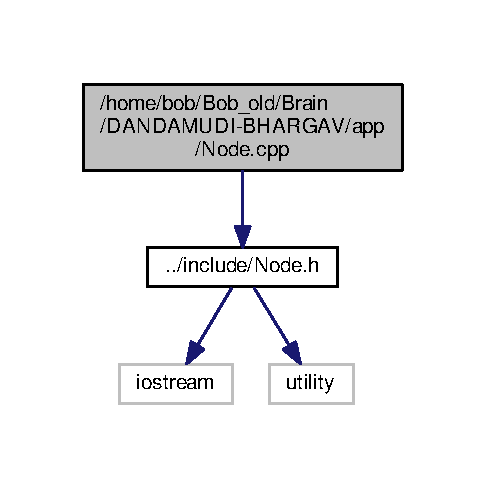
\includegraphics[width=206pt]{Node_8cpp__incl}
\end{center}
\end{figure}


\subsection{Detailed Description}
Basic \hyperlink{structNode}{Node} structure definition with 2 constructors. 

\begin{DoxyAuthor}{Author}
Bhargav Dandamudi 
\end{DoxyAuthor}
\begin{DoxyVersion}{Version}
1 
\end{DoxyVersion}
\begin{DoxyDate}{Date}
2019-\/04-\/03 
\end{DoxyDate}

\hypertarget{optimalPlanner_8cpp}{}\section{/home/bob/\+Bob\+\_\+old/\+Brain/\+Discrete\+\_\+\+Planners/app/optimal\+Planner.cpp File Reference}
\label{optimalPlanner_8cpp}\index{/home/bob/\+Bob\+\_\+old/\+Brain/\+Discrete\+\_\+\+Planners/app/optimal\+Planner.\+cpp@{/home/bob/\+Bob\+\_\+old/\+Brain/\+Discrete\+\_\+\+Planners/app/optimal\+Planner.\+cpp}}


Astar Algorithm A$\ast$ Search Algorithm\+: At each step it picks the node according to a value-\/‘f’ which is a parameter equal to the sum of two other parameters – ‘g’ and ‘h’. At each step it picks the node/cell having the lowest ‘f’, and process that node/cell. g cost = the movement cost to move from the starting point to a given node on the grid, following the path generated to get there. h cost = the estimated movement cost to move from that given node on the grid to the final destination.  


{\ttfamily \#include \char`\"{}../include/optimal\+Planner.\+h\char`\"{}}\\*
{\ttfamily \#include \char`\"{}../include/node.\+h\char`\"{}}\\*
Include dependency graph for optimal\+Planner.\+cpp\+:
\nopagebreak
\begin{figure}[H]
\begin{center}
\leavevmode
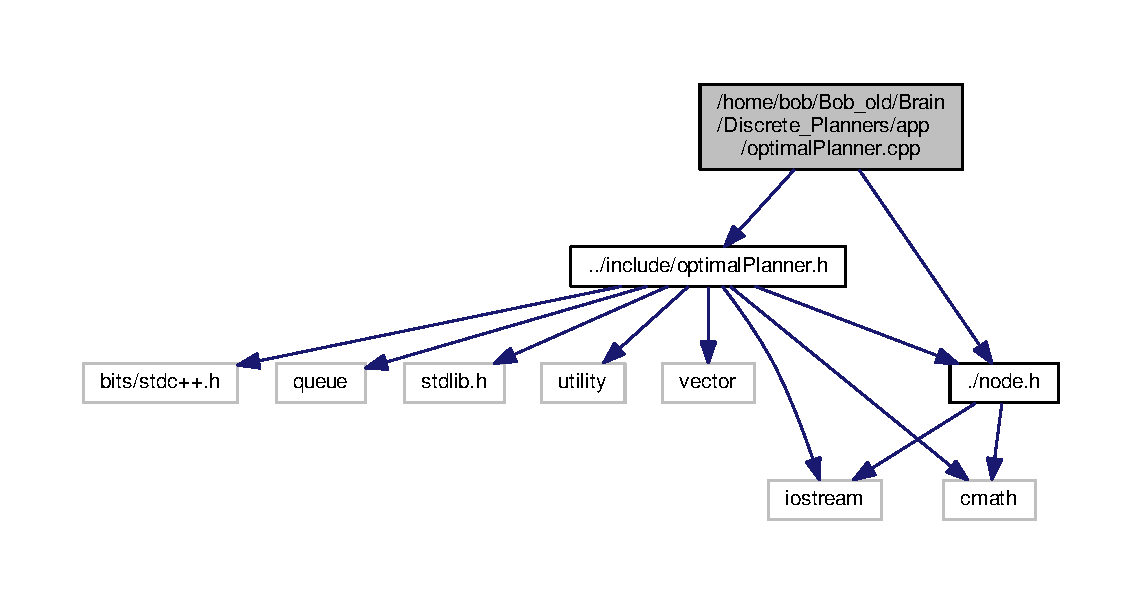
\includegraphics[width=350pt]{optimalPlanner_8cpp__incl}
\end{center}
\end{figure}


\subsection{Detailed Description}
Astar Algorithm A$\ast$ Search Algorithm\+: At each step it picks the node according to a value-\/‘f’ which is a parameter equal to the sum of two other parameters – ‘g’ and ‘h’. At each step it picks the node/cell having the lowest ‘f’, and process that node/cell. g cost = the movement cost to move from the starting point to a given node on the grid, following the path generated to get there. h cost = the estimated movement cost to move from that given node on the grid to the final destination. 

Here we are using Manhattan Distance for calculating h cost for each nodes

Working\+:
\begin{DoxyEnumerate}
\item Add the starting node (or node) to the open list.
\item Repeat the following\+:
\end{DoxyEnumerate}

A) Look for the lowest F cost node on the open list. We refer to this as the current node.

B). Switch it to the closed list.

C) For each of the 4 nodes adjacent to this current node …

If it is not walkable or if it is on the closed list, ignore it. Otherwise do the following. If it isn’t on the open list, add it to the open list. Make the current node the parent of this node. Record the F, G, and H costs of the node. If it is on the open list already, check to see if this path to that node is better, using G cost as the measure. A lower G cost means that this is a better path. If so, change the parent of the node to the current node, and recalculate the G and F scores of the node. If you are keeping your open list sorted by F score, you may need to resort the list to account for the change. D) Stop when you\+:

Add the target node to the closed list, in which case the path has been found, or Fail to find the target node, and the open list is empty. In this case, there is no path.
\begin{DoxyEnumerate}
\item Save the path. Working backwards from the target node, go from each node to its parent node until you reach the starting node. That is your path.

\begin{DoxyAuthor}{Author}
Bhargav Dandamudi 
\end{DoxyAuthor}
\begin{DoxyVersion}{Version}
1 
\end{DoxyVersion}
\begin{DoxyDate}{Date}
2019-\/04-\/04 
\end{DoxyDate}

\end{DoxyEnumerate}
\hypertarget{RandomPlanner_8cpp}{}\section{/home/bob/\+Bob\+\_\+old/\+Brain/\+Discrete\+\_\+\+Planners/app/\+Random\+Planner.cpp File Reference}
\label{RandomPlanner_8cpp}\index{/home/bob/\+Bob\+\_\+old/\+Brain/\+Discrete\+\_\+\+Planners/app/\+Random\+Planner.\+cpp@{/home/bob/\+Bob\+\_\+old/\+Brain/\+Discrete\+\_\+\+Planners/app/\+Random\+Planner.\+cpp}}


Random Planner class definitions.  


{\ttfamily \#include \char`\"{}../include/\+Random\+Planner.\+h\char`\"{}}\\*
{\ttfamily \#include \char`\"{}../include/\+Node.\+h\char`\"{}}\\*
Include dependency graph for Random\+Planner.\+cpp\+:
\nopagebreak
\begin{figure}[H]
\begin{center}
\leavevmode
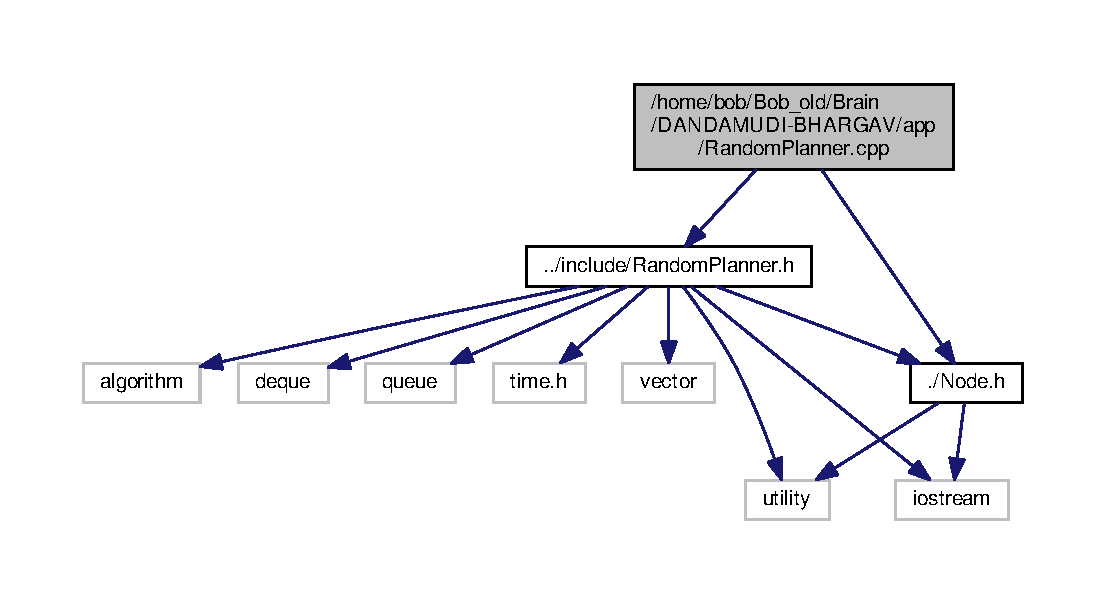
\includegraphics[width=350pt]{RandomPlanner_8cpp__incl}
\end{center}
\end{figure}


\subsection{Detailed Description}
Random Planner class definitions. 

\begin{DoxyAuthor}{Author}
Bhargav Dandamudi 
\end{DoxyAuthor}
\begin{DoxyVersion}{Version}
1 
\end{DoxyVersion}
\begin{DoxyDate}{Date}
2019-\/04-\/03 
\end{DoxyDate}

\hypertarget{Node_8h}{}\section{/home/bob/\+Bob\+\_\+old/\+Brain/\+D\+A\+N\+D\+A\+M\+U\+D\+I-\/\+B\+H\+A\+R\+G\+A\+V/include/\+Node.h File Reference}
\label{Node_8h}\index{/home/bob/\+Bob\+\_\+old/\+Brain/\+D\+A\+N\+D\+A\+M\+U\+D\+I-\/\+B\+H\+A\+R\+G\+A\+V/include/\+Node.\+h@{/home/bob/\+Bob\+\_\+old/\+Brain/\+D\+A\+N\+D\+A\+M\+U\+D\+I-\/\+B\+H\+A\+R\+G\+A\+V/include/\+Node.\+h}}


A structure to denote each block in map for \hyperlink{classRandomPlanner}{Random\+Planner}.  


{\ttfamily \#include $<$iostream$>$}\\*
{\ttfamily \#include $<$utility$>$}\\*
Include dependency graph for Node.\+h\+:
\nopagebreak
\begin{figure}[H]
\begin{center}
\leavevmode
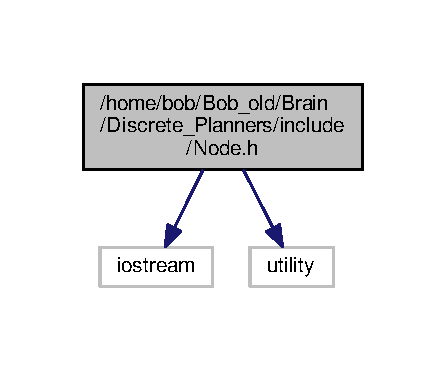
\includegraphics[width=248pt]{Node_8h__incl}
\end{center}
\end{figure}
This graph shows which files directly or indirectly include this file\+:
\nopagebreak
\begin{figure}[H]
\begin{center}
\leavevmode
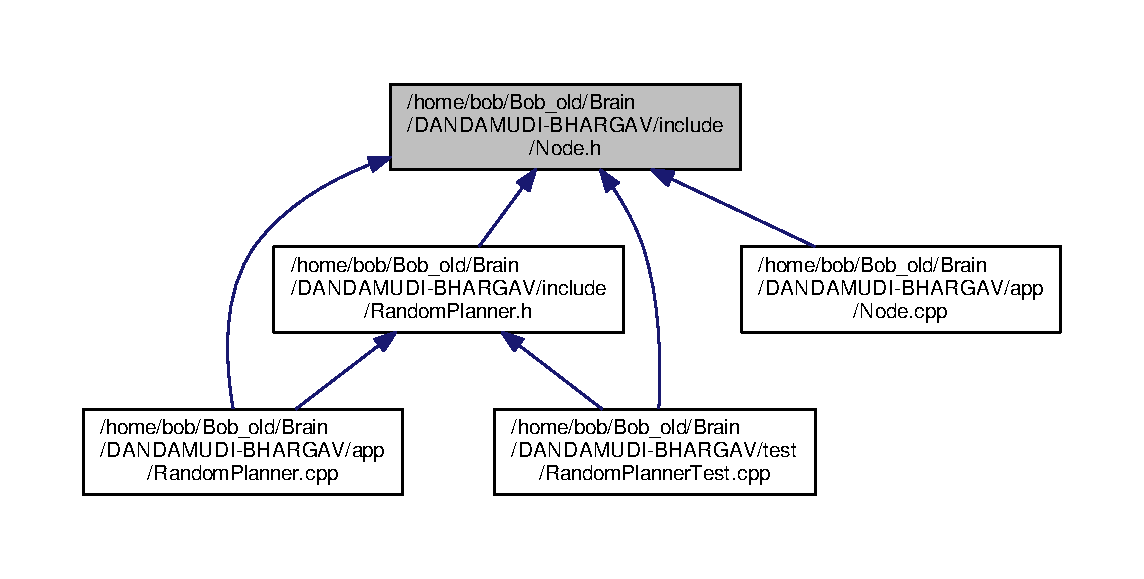
\includegraphics[width=350pt]{Node_8h__dep__incl}
\end{center}
\end{figure}
\subsection*{Classes}
\begin{DoxyCompactItemize}
\item 
struct \hyperlink{structNode}{Node}
\begin{DoxyCompactList}\small\item\em Basic \hyperlink{structNode}{Node} Structure for each block. \end{DoxyCompactList}\end{DoxyCompactItemize}


\subsection{Detailed Description}
A structure to denote each block in map for \hyperlink{classRandomPlanner}{Random\+Planner}. 

\begin{DoxyAuthor}{Author}
Bhargav Dandamudi 
\end{DoxyAuthor}
\begin{DoxyVersion}{Version}
1 
\end{DoxyVersion}
\begin{DoxyDate}{Date}
2019-\/04-\/03 
\end{DoxyDate}

\hypertarget{node_8h}{}\section{/home/bob/\+Bob\+\_\+old/\+Brain/\+Discrete\+\_\+\+Planners/include/node.h File Reference}
\label{node_8h}\index{/home/bob/\+Bob\+\_\+old/\+Brain/\+Discrete\+\_\+\+Planners/include/node.\+h@{/home/bob/\+Bob\+\_\+old/\+Brain/\+Discrete\+\_\+\+Planners/include/node.\+h}}


data structure for containing optimal planner nodes  


{\ttfamily \#include $<$cmath$>$}\\*
{\ttfamily \#include $<$iostream$>$}\\*
Include dependency graph for node.\+h\+:
\nopagebreak
\begin{figure}[H]
\begin{center}
\leavevmode
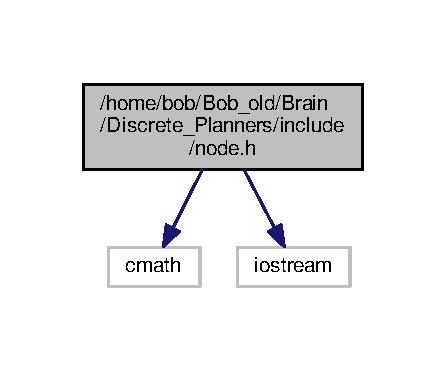
\includegraphics[width=214pt]{node_8h__incl}
\end{center}
\end{figure}
This graph shows which files directly or indirectly include this file\+:
\nopagebreak
\begin{figure}[H]
\begin{center}
\leavevmode
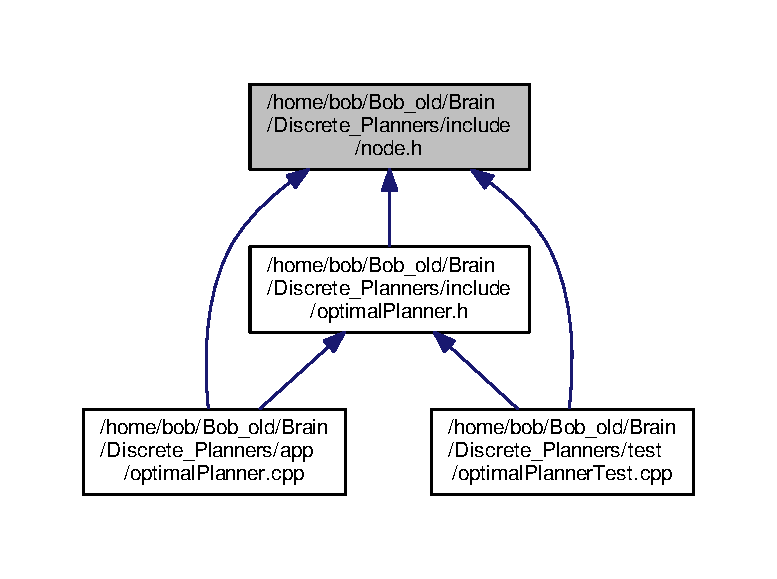
\includegraphics[width=350pt]{node_8h__dep__incl}
\end{center}
\end{figure}
\subsection*{Classes}
\begin{DoxyCompactItemize}
\item 
struct \hyperlink{structnode}{node}
\begin{DoxyCompactList}\small\item\em node which contains location, parent location and f g and h cost of the node \end{DoxyCompactList}\end{DoxyCompactItemize}


\subsection{Detailed Description}
data structure for containing optimal planner nodes 

\begin{DoxyAuthor}{Author}
Bhargav Dandamudi 
\end{DoxyAuthor}
\begin{DoxyVersion}{Version}
1 
\end{DoxyVersion}
\begin{DoxyDate}{Date}
2019-\/04-\/03 
\end{DoxyDate}

\hypertarget{optimalPlanner_8h}{}\section{/home/bob/\+Bob\+\_\+old/\+Brain/\+Discrete\+\_\+\+Planners/include/optimal\+Planner.h File Reference}
\label{optimalPlanner_8h}\index{/home/bob/\+Bob\+\_\+old/\+Brain/\+Discrete\+\_\+\+Planners/include/optimal\+Planner.\+h@{/home/bob/\+Bob\+\_\+old/\+Brain/\+Discrete\+\_\+\+Planners/include/optimal\+Planner.\+h}}


Optimal Planner using astar algorithm to reach goal.  


{\ttfamily \#include \char`\"{}./node.\+h\char`\"{}}\\*
{\ttfamily \#include $<$bits/stdc++.\+h$>$}\\*
{\ttfamily \#include $<$cmath$>$}\\*
{\ttfamily \#include $<$iostream$>$}\\*
{\ttfamily \#include $<$queue$>$}\\*
{\ttfamily \#include $<$stdlib.\+h$>$}\\*
{\ttfamily \#include $<$utility$>$}\\*
{\ttfamily \#include $<$vector$>$}\\*
Include dependency graph for optimal\+Planner.\+h\+:
\nopagebreak
\begin{figure}[H]
\begin{center}
\leavevmode
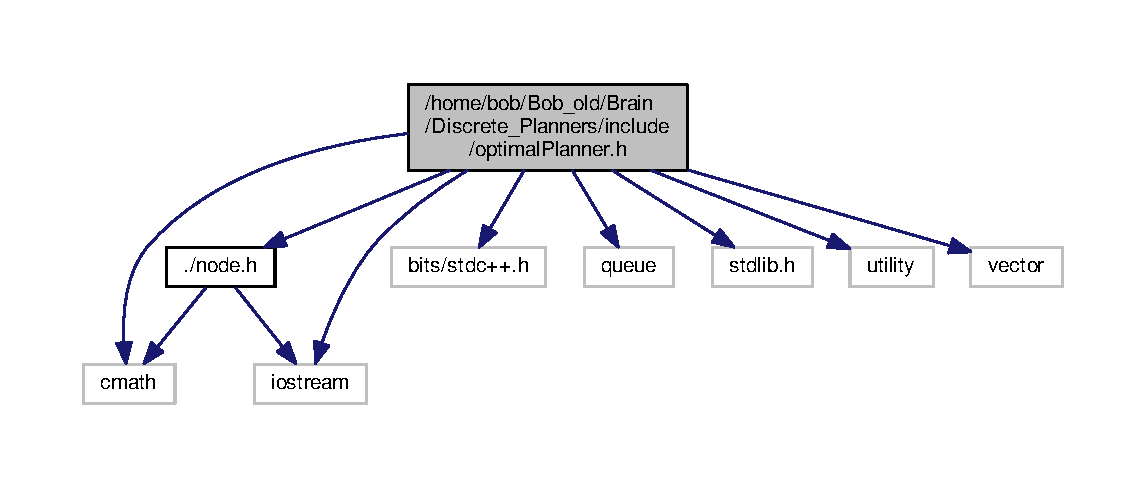
\includegraphics[width=350pt]{optimalPlanner_8h__incl}
\end{center}
\end{figure}
This graph shows which files directly or indirectly include this file\+:
\nopagebreak
\begin{figure}[H]
\begin{center}
\leavevmode
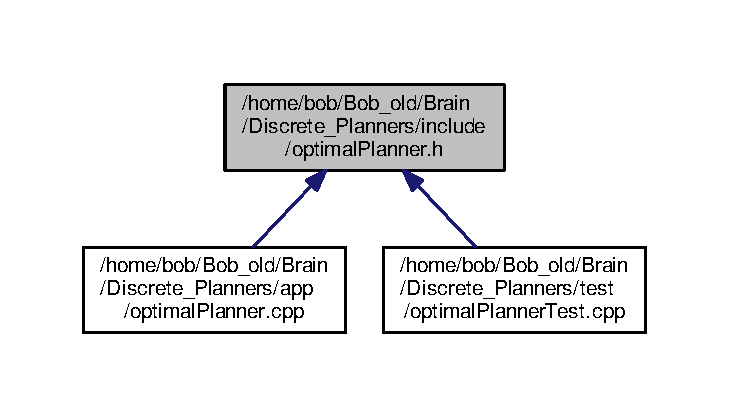
\includegraphics[width=350pt]{optimalPlanner_8h__dep__incl}
\end{center}
\end{figure}
\subsection*{Classes}
\begin{DoxyCompactItemize}
\item 
class \hyperlink{classoptimalPlanner}{optimal\+Planner}
\begin{DoxyCompactList}\small\item\em Optimal Planner class members declaration we are using Astar algorithm for finding optimal path. \end{DoxyCompactList}\end{DoxyCompactItemize}
\subsection*{Typedefs}
\begin{DoxyCompactItemize}
\item 
typedef std\+::pair$<$ double, std\+::pair$<$ int, int $>$ $>$ {\bfseries Double\+Pair}\hypertarget{optimalPlanner_8h_a50e8424011e2ee22d906b27f574d2a5d}{}\label{optimalPlanner_8h_a50e8424011e2ee22d906b27f574d2a5d}

\end{DoxyCompactItemize}


\subsection{Detailed Description}
Optimal Planner using astar algorithm to reach goal. 

\begin{DoxyAuthor}{Author}
Bhargav Dandamudi 
\end{DoxyAuthor}
\begin{DoxyVersion}{Version}
1 
\end{DoxyVersion}
\begin{DoxyDate}{Date}
2019-\/04-\/04 
\end{DoxyDate}

\hypertarget{RandomPlanner_8h}{}\section{/home/bob/\+Bob\+\_\+old/\+Brain/\+Discrete\+\_\+\+Planners/include/\+Random\+Planner.h File Reference}
\label{RandomPlanner_8h}\index{/home/bob/\+Bob\+\_\+old/\+Brain/\+Discrete\+\_\+\+Planners/include/\+Random\+Planner.\+h@{/home/bob/\+Bob\+\_\+old/\+Brain/\+Discrete\+\_\+\+Planners/include/\+Random\+Planner.\+h}}


Main Random Discrete Planner Class with all declarations.  


{\ttfamily \#include \char`\"{}./\+Node.\+h\char`\"{}}\\*
{\ttfamily \#include $<$algorithm$>$}\\*
{\ttfamily \#include $<$deque$>$}\\*
{\ttfamily \#include $<$iostream$>$}\\*
{\ttfamily \#include $<$queue$>$}\\*
{\ttfamily \#include $<$time.\+h$>$}\\*
{\ttfamily \#include $<$utility$>$}\\*
{\ttfamily \#include $<$vector$>$}\\*
Include dependency graph for Random\+Planner.\+h\+:
\nopagebreak
\begin{figure}[H]
\begin{center}
\leavevmode
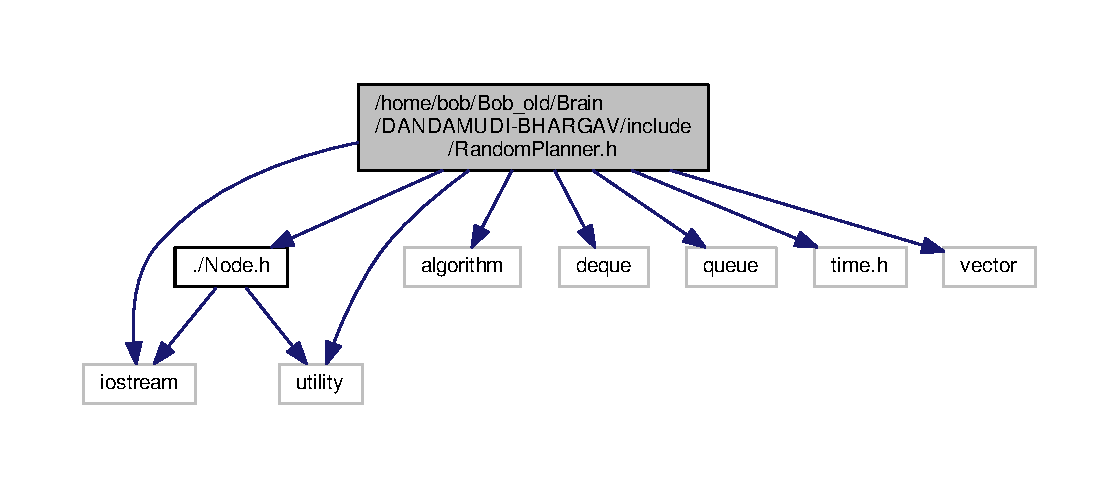
\includegraphics[width=350pt]{RandomPlanner_8h__incl}
\end{center}
\end{figure}
This graph shows which files directly or indirectly include this file\+:
\nopagebreak
\begin{figure}[H]
\begin{center}
\leavevmode
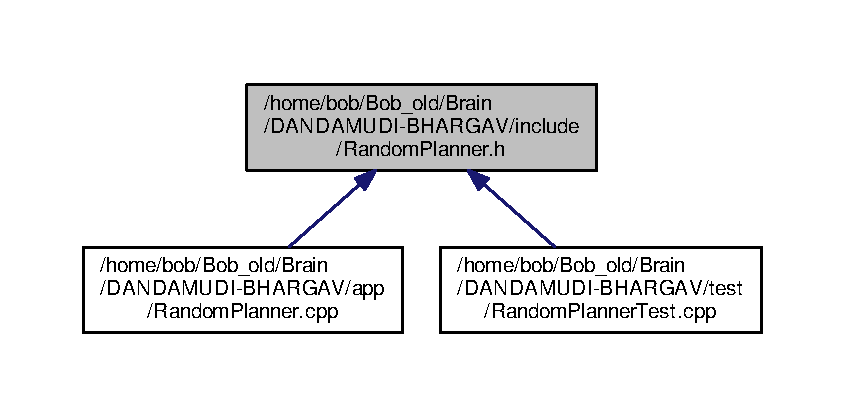
\includegraphics[width=350pt]{RandomPlanner_8h__dep__incl}
\end{center}
\end{figure}
\subsection*{Classes}
\begin{DoxyCompactItemize}
\item 
class \hyperlink{classRandomPlanner}{Random\+Planner}
\begin{DoxyCompactList}\small\item\em The random planner tries to find a path to the goal by randomly moving in the environment (only orthogonal moves are legal). If the planner can not find an acceptable solution in less than max\+\_\+step\+\_\+number, the search should fail. The random planner, while being erratic, has a short memory, and it will never attempt to visit a cell that was visited in the last sqrt(max\+\_\+step\+\_\+number) steps except if this is the only available option. \end{DoxyCompactList}\end{DoxyCompactItemize}


\subsection{Detailed Description}
Main Random Discrete Planner Class with all declarations. 

\begin{DoxyAuthor}{Author}
Bhargav Dandamudi 
\end{DoxyAuthor}
\begin{DoxyVersion}{Version}
1 
\end{DoxyVersion}
\begin{DoxyDate}{Date}
2019-\/04-\/03 
\end{DoxyDate}

\hypertarget{optimalPlannerTest_8cpp}{}\section{/home/bob/\+Bob\+\_\+old/\+Brain/\+D\+A\+N\+D\+A\+M\+U\+D\+I-\/\+B\+H\+A\+R\+G\+A\+V/test/optimal\+Planner\+Test.cpp File Reference}
\label{optimalPlannerTest_8cpp}\index{/home/bob/\+Bob\+\_\+old/\+Brain/\+D\+A\+N\+D\+A\+M\+U\+D\+I-\/\+B\+H\+A\+R\+G\+A\+V/test/optimal\+Planner\+Test.\+cpp@{/home/bob/\+Bob\+\_\+old/\+Brain/\+D\+A\+N\+D\+A\+M\+U\+D\+I-\/\+B\+H\+A\+R\+G\+A\+V/test/optimal\+Planner\+Test.\+cpp}}


Test Optimal Test functions.  


{\ttfamily \#include \char`\"{}../include/optimal\+Planner.\+h\char`\"{}}\\*
{\ttfamily \#include \char`\"{}../include/node.\+h\char`\"{}}\\*
{\ttfamily \#include $<$gtest/gtest.\+h$>$}\\*
Include dependency graph for optimal\+Planner\+Test.\+cpp\+:
\nopagebreak
\begin{figure}[H]
\begin{center}
\leavevmode
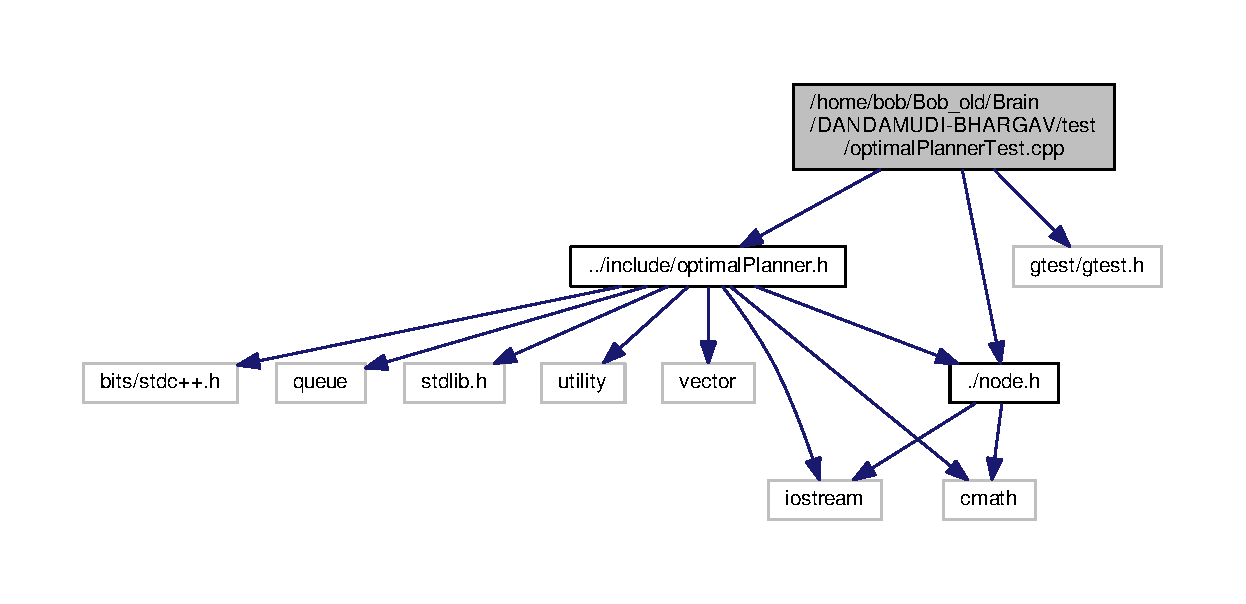
\includegraphics[width=350pt]{optimalPlannerTest_8cpp__incl}
\end{center}
\end{figure}
\subsection*{Functions}
\begin{DoxyCompactItemize}
\item 
std\+::pair$<$ int, int $>$ {\bfseries robot\+\_\+pose} (2, 0)\hypertarget{optimalPlannerTest_8cpp_af42021b64a9d82c0364c3d21ebab711a}{}\label{optimalPlannerTest_8cpp_af42021b64a9d82c0364c3d21ebab711a}

\item 
std\+::pair$<$ int, int $>$ {\bfseries goal\+\_\+pose} (5, 5)\hypertarget{optimalPlannerTest_8cpp_a0eb13ebb80bf411a8efdb07fffd36393}{}\label{optimalPlannerTest_8cpp_a0eb13ebb80bf411a8efdb07fffd36393}

\item 
{\bfseries T\+E\+ST} (test, invalidity\+Test)\hypertarget{optimalPlannerTest_8cpp_a222fac85631da7649c800556c441d02e}{}\label{optimalPlannerTest_8cpp_a222fac85631da7649c800556c441d02e}

\item 
{\bfseries T\+E\+ST} (test, On\+Boundary\+Validity\+Test)\hypertarget{optimalPlannerTest_8cpp_a71aa467392d0ba1ea1d2b93b74bae23c}{}\label{optimalPlannerTest_8cpp_a71aa467392d0ba1ea1d2b93b74bae23c}

\item 
{\bfseries T\+E\+ST} (test, validity\+Test)\hypertarget{optimalPlannerTest_8cpp_a8a7be640b9f0b721d97258e15986d22a}{}\label{optimalPlannerTest_8cpp_a8a7be640b9f0b721d97258e15986d22a}

\item 
{\bfseries T\+E\+ST} (test, goal\+Point\+Registering)\hypertarget{optimalPlannerTest_8cpp_ab46e99ce2127bb1dfc3410f00d196765}{}\label{optimalPlannerTest_8cpp_ab46e99ce2127bb1dfc3410f00d196765}

\item 
{\bfseries T\+E\+ST} (test, starting\+Point\+Registering)\hypertarget{optimalPlannerTest_8cpp_ac9ebf71157c06f21a78434c616dd34e2}{}\label{optimalPlannerTest_8cpp_ac9ebf71157c06f21a78434c616dd34e2}

\item 
{\bfseries T\+E\+ST} (test, ylength\+Test)\hypertarget{optimalPlannerTest_8cpp_a687cc51b1615c757dcffb3c680bd366c}{}\label{optimalPlannerTest_8cpp_a687cc51b1615c757dcffb3c680bd366c}

\item 
{\bfseries T\+E\+ST} (test, xlength\+Test)\hypertarget{optimalPlannerTest_8cpp_ac7468cc723dde8b63174ca1e21636c54}{}\label{optimalPlannerTest_8cpp_ac7468cc723dde8b63174ca1e21636c54}

\item 
{\bfseries T\+E\+ST} (test, is\+Blocked\+Test)\hypertarget{optimalPlannerTest_8cpp_a7cfde340f22cbfb5f62c64b5a8b41d1b}{}\label{optimalPlannerTest_8cpp_a7cfde340f22cbfb5f62c64b5a8b41d1b}

\item 
{\bfseries T\+E\+ST} (test, is\+It\+Goal\+Yet\+Test)\hypertarget{optimalPlannerTest_8cpp_ac49a7152f8e66c58cf3de1d0f1fc7740}{}\label{optimalPlannerTest_8cpp_ac49a7152f8e66c58cf3de1d0f1fc7740}

\item 
{\bfseries T\+E\+ST} (test, is\+Goal\+Yet\+Test)\hypertarget{optimalPlannerTest_8cpp_ad37cd04817813a2455041b7a1ea585bf}{}\label{optimalPlannerTest_8cpp_ad37cd04817813a2455041b7a1ea585bf}

\item 
{\bfseries T\+E\+ST} (test, calculate\+H\+Cost\+Test)\hypertarget{optimalPlannerTest_8cpp_a3c708181d70aff4e54cc282d288f7186}{}\label{optimalPlannerTest_8cpp_a3c708181d70aff4e54cc282d288f7186}

\item 
{\bfseries T\+E\+ST} (test, go\+Top\+Test)\hypertarget{optimalPlannerTest_8cpp_a87c978de0861976875d8b9ef04bdbcf5}{}\label{optimalPlannerTest_8cpp_a87c978de0861976875d8b9ef04bdbcf5}

\item 
{\bfseries T\+E\+ST} (test, go\+Down\+Test)\hypertarget{optimalPlannerTest_8cpp_ae19a1225fc785a9c8daa84565a334105}{}\label{optimalPlannerTest_8cpp_ae19a1225fc785a9c8daa84565a334105}

\item 
{\bfseries T\+E\+ST} (test, go\+Left\+Test)\hypertarget{optimalPlannerTest_8cpp_a7608407d40bab6a7c8c83547b0d04943}{}\label{optimalPlannerTest_8cpp_a7608407d40bab6a7c8c83547b0d04943}

\item 
{\bfseries T\+E\+ST} (test, go\+Right\+Test)\hypertarget{optimalPlannerTest_8cpp_a37cdd917f654f20eb2860c9b98899047}{}\label{optimalPlannerTest_8cpp_a37cdd917f654f20eb2860c9b98899047}

\item 
{\bfseries T\+E\+ST} (test, move\+And\+Update\+Nodes\+Test)\hypertarget{optimalPlannerTest_8cpp_ab757308d9bc166eb05e3c9976872e585}{}\label{optimalPlannerTest_8cpp_ab757308d9bc166eb05e3c9976872e585}

\item 
{\bfseries T\+E\+ST} (test, move\+And\+Update\+Nodes\+H\+C\+Test)\hypertarget{optimalPlannerTest_8cpp_a24eb8f74356d081a0689c4d70005f27c}{}\label{optimalPlannerTest_8cpp_a24eb8f74356d081a0689c4d70005f27c}

\item 
{\bfseries T\+E\+ST} (test, move\+And\+Update\+Nodes\+G\+C\+Test)\hypertarget{optimalPlannerTest_8cpp_a92f5a5b9b8302f8c229f937834f62734}{}\label{optimalPlannerTest_8cpp_a92f5a5b9b8302f8c229f937834f62734}

\item 
{\bfseries T\+E\+ST} (test, move\+And\+Update\+Nodes\+Parent\+Test)\hypertarget{optimalPlannerTest_8cpp_aaa2b53890b444c826ee452dccd9f0c8c}{}\label{optimalPlannerTest_8cpp_aaa2b53890b444c826ee452dccd9f0c8c}

\item 
{\bfseries T\+E\+ST} (test, path\+Test)\hypertarget{optimalPlannerTest_8cpp_a7ead2373c74c7fed67fc446ee7716f35}{}\label{optimalPlannerTest_8cpp_a7ead2373c74c7fed67fc446ee7716f35}

\end{DoxyCompactItemize}
\subsection*{Variables}
\begin{DoxyCompactItemize}
\item 
std\+::vector$<$ std\+::vector$<$ int $>$ $>$ {\bfseries world\+\_\+state}
\item 
\hyperlink{classoptimalPlanner}{optimal\+Planner} {\bfseries test\+Obj} (world\+\_\+state, robot\+\_\+pose, goal\+\_\+pose)\hypertarget{optimalPlannerTest_8cpp_a1a65f637defbccb6716246a4e38e5fb9}{}\label{optimalPlannerTest_8cpp_a1a65f637defbccb6716246a4e38e5fb9}

\end{DoxyCompactItemize}


\subsection{Detailed Description}
Test Optimal Test functions. 

\begin{DoxyAuthor}{Author}
Bhargav Dandamudi 
\end{DoxyAuthor}
\begin{DoxyVersion}{Version}
1 
\end{DoxyVersion}
\begin{DoxyDate}{Date}
2019-\/04-\/05 
\end{DoxyDate}


\subsection{Variable Documentation}
\index{optimal\+Planner\+Test.\+cpp@{optimal\+Planner\+Test.\+cpp}!world\+\_\+state@{world\+\_\+state}}
\index{world\+\_\+state@{world\+\_\+state}!optimal\+Planner\+Test.\+cpp@{optimal\+Planner\+Test.\+cpp}}
\subsubsection[{\texorpdfstring{world\+\_\+state}{world_state}}]{\setlength{\rightskip}{0pt plus 5cm}std\+::vector$<$std\+::vector$<$int$>$ $>$ world\+\_\+state}\hypertarget{optimalPlannerTest_8cpp_a4c2a83af452fd23aea729a5f1e9dd309}{}\label{optimalPlannerTest_8cpp_a4c2a83af452fd23aea729a5f1e9dd309}
{\bfseries Initial value\+:}
\begin{DoxyCode}
\{
    \{0, 0, 1, 0, 0, 0\}, \{0, 0, 1, 0, 0, 0\}, \{0, 0, 0, 0, 1, 0\},
    \{0, 0, 0, 0, 1, 0\}, \{0, 0, 1, 1, 1, 0\}, \{0, 0, 0, 0, 0, 0\}\}
\end{DoxyCode}

\hypertarget{RandomPlannerTest_8cpp}{}\section{/home/bob/\+Bob\+\_\+old/\+Brain/\+D\+A\+N\+D\+A\+M\+U\+D\+I-\/\+B\+H\+A\+R\+G\+A\+V/test/\+Random\+Planner\+Test.cpp File Reference}
\label{RandomPlannerTest_8cpp}\index{/home/bob/\+Bob\+\_\+old/\+Brain/\+D\+A\+N\+D\+A\+M\+U\+D\+I-\/\+B\+H\+A\+R\+G\+A\+V/test/\+Random\+Planner\+Test.\+cpp@{/home/bob/\+Bob\+\_\+old/\+Brain/\+D\+A\+N\+D\+A\+M\+U\+D\+I-\/\+B\+H\+A\+R\+G\+A\+V/test/\+Random\+Planner\+Test.\+cpp}}


To test all functions in Random P\+Lanner.  


{\ttfamily \#include \char`\"{}../include/\+Random\+Planner.\+h\char`\"{}}\\*
{\ttfamily \#include \char`\"{}../include/\+Node.\+h\char`\"{}}\\*
{\ttfamily \#include $<$gtest/gtest.\+h$>$}\\*
Include dependency graph for Random\+Planner\+Test.\+cpp\+:
\nopagebreak
\begin{figure}[H]
\begin{center}
\leavevmode
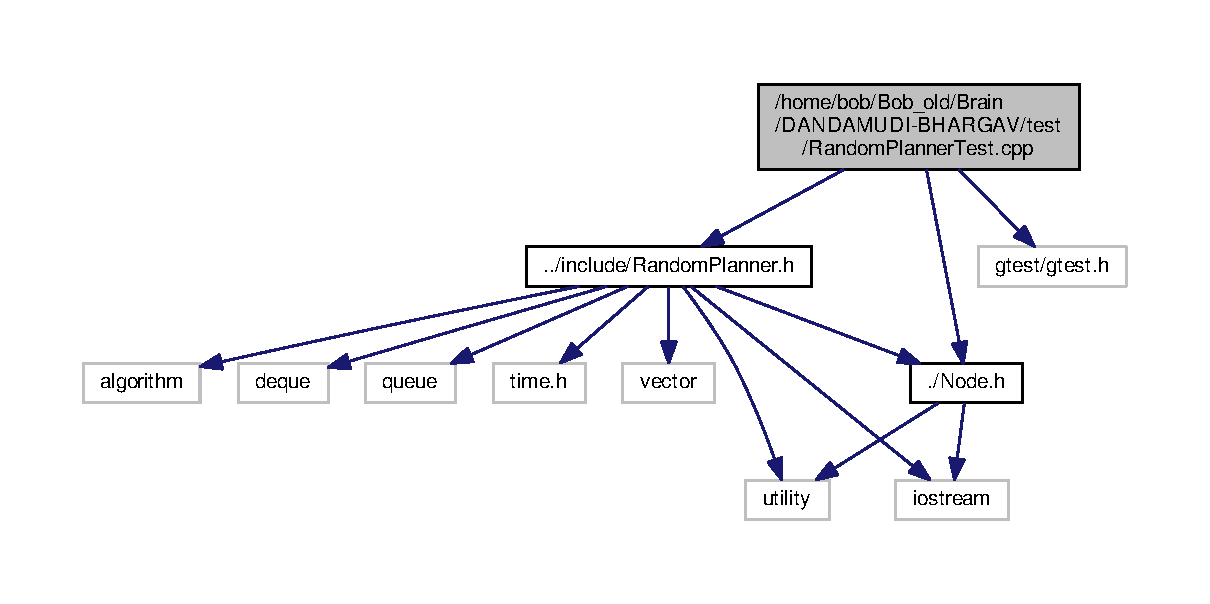
\includegraphics[width=350pt]{RandomPlannerTest_8cpp__incl}
\end{center}
\end{figure}
\subsection*{Functions}
\begin{DoxyCompactItemize}
\item 
std\+::pair$<$ int, int $>$ {\bfseries robot\+\_\+pose\+\_\+rp} (2, 0)\hypertarget{RandomPlannerTest_8cpp_a3e51cc7adea1ed184ccb32e9e957d737}{}\label{RandomPlannerTest_8cpp_a3e51cc7adea1ed184ccb32e9e957d737}

\item 
std\+::pair$<$ int, int $>$ {\bfseries goal\+\_\+pose\+\_\+rp} (5, 5)\hypertarget{RandomPlannerTest_8cpp_a971837d09232d17581e856492b7aa844}{}\label{RandomPlannerTest_8cpp_a971837d09232d17581e856492b7aa844}

\item 
{\bfseries T\+E\+ST} (random\+Test, goal\+Point\+Set\+T\+Est)\hypertarget{RandomPlannerTest_8cpp_a012d3595c4e402ac0a2fd959ecb19b6c}{}\label{RandomPlannerTest_8cpp_a012d3595c4e402ac0a2fd959ecb19b6c}

\item 
{\bfseries T\+E\+ST} (random\+Test, start\+Point\+Test)\hypertarget{RandomPlannerTest_8cpp_aa4d323749f54774e9943aaea418e6bca}{}\label{RandomPlannerTest_8cpp_aa4d323749f54774e9943aaea418e6bca}

\item 
{\bfseries T\+E\+ST} (random\+Test, Is\+Obstacle\+Test)\hypertarget{RandomPlannerTest_8cpp_af704b5c16bf34fd5dc3285c657b65210}{}\label{RandomPlannerTest_8cpp_af704b5c16bf34fd5dc3285c657b65210}

\item 
{\bfseries T\+E\+ST} (random\+Test, Is\+Obstacleinside\+Test)\hypertarget{RandomPlannerTest_8cpp_a9e63e24776f8b074316fbd866d82f272}{}\label{RandomPlannerTest_8cpp_a9e63e24776f8b074316fbd866d82f272}

\item 
{\bfseries T\+E\+ST} (random\+Test, Is\+Obstacle\+Outside\+Test)\hypertarget{RandomPlannerTest_8cpp_ae590db2e582dee17c36ec571b49964fd}{}\label{RandomPlannerTest_8cpp_ae590db2e582dee17c36ec571b49964fd}

\item 
{\bfseries T\+E\+ST} (random\+Test, Xlength\+T\+E\+S\+T\+\_\+\+Rp)\hypertarget{RandomPlannerTest_8cpp_a7c9b2cc058cb307848096ee18cf04356}{}\label{RandomPlannerTest_8cpp_a7c9b2cc058cb307848096ee18cf04356}

\item 
{\bfseries T\+E\+ST} (random\+Test, Ylength\+T\+E\+S\+T\+\_\+\+Rp)\hypertarget{RandomPlannerTest_8cpp_aa3885a8326dd812deef79a46d063b489}{}\label{RandomPlannerTest_8cpp_aa3885a8326dd812deef79a46d063b489}

\item 
{\bfseries T\+E\+ST} (random\+Test, Move\+Top)\hypertarget{RandomPlannerTest_8cpp_a974889ada7c73d695cd796e7a8982cde}{}\label{RandomPlannerTest_8cpp_a974889ada7c73d695cd796e7a8982cde}

\item 
{\bfseries T\+E\+ST} (random\+Test, Move\+Left)\hypertarget{RandomPlannerTest_8cpp_a5c9dad2d6b7febea2dbecb74ef0280e4}{}\label{RandomPlannerTest_8cpp_a5c9dad2d6b7febea2dbecb74ef0280e4}

\item 
{\bfseries T\+E\+ST} (random\+Test, Move\+Down)\hypertarget{RandomPlannerTest_8cpp_a599e1118674002909c4550f9f4712a49}{}\label{RandomPlannerTest_8cpp_a599e1118674002909c4550f9f4712a49}

\item 
{\bfseries T\+E\+ST} (random\+Test, Move\+Right)\hypertarget{RandomPlannerTest_8cpp_a223228bf165625ddabeff6f24f82dd51}{}\label{RandomPlannerTest_8cpp_a223228bf165625ddabeff6f24f82dd51}

\item 
{\bfseries T\+E\+ST} (random\+Test, find\+Neighbors\+Test)\hypertarget{RandomPlannerTest_8cpp_a032050cff7b692df6971d9ca7cf3f814}{}\label{RandomPlannerTest_8cpp_a032050cff7b692df6971d9ca7cf3f814}

\end{DoxyCompactItemize}
\subsection*{Variables}
\begin{DoxyCompactItemize}
\item 
std\+::vector$<$ std\+::vector$<$ int $>$ $>$ {\bfseries world}
\item 
\hyperlink{classRandomPlanner}{Random\+Planner} {\bfseries rp\+\_\+test} (world, robot\+\_\+pose\+\_\+rp, goal\+\_\+pose\+\_\+rp)\hypertarget{RandomPlannerTest_8cpp_a1dd1558b1cad19a77d061dd2284ac320}{}\label{RandomPlannerTest_8cpp_a1dd1558b1cad19a77d061dd2284ac320}

\end{DoxyCompactItemize}


\subsection{Detailed Description}
To test all functions in Random P\+Lanner. 

\begin{DoxyAuthor}{Author}
Bhargav Dandamudi 
\end{DoxyAuthor}
\begin{DoxyVersion}{Version}
1 
\end{DoxyVersion}
\begin{DoxyDate}{Date}
2019-\/04-\/05 
\end{DoxyDate}


\subsection{Variable Documentation}
\index{Random\+Planner\+Test.\+cpp@{Random\+Planner\+Test.\+cpp}!world@{world}}
\index{world@{world}!Random\+Planner\+Test.\+cpp@{Random\+Planner\+Test.\+cpp}}
\subsubsection[{\texorpdfstring{world}{world}}]{\setlength{\rightskip}{0pt plus 5cm}std\+::vector$<$std\+::vector$<$int$>$ $>$ world}\hypertarget{RandomPlannerTest_8cpp_a5d78825b6562fcb45c8dd3645c21266e}{}\label{RandomPlannerTest_8cpp_a5d78825b6562fcb45c8dd3645c21266e}
{\bfseries Initial value\+:}
\begin{DoxyCode}
\{\{0, 0, 1, 0, 0, 0\}, \{0, 0, 1, 0, 0, 0\},
                                    \{0, 0, 0, 0, 1, 0\}, \{0, 0, 0, 0, 1, 0\},
                                    \{0, 0, 1, 1, 1, 0\}, \{0, 0, 0, 0, 0, 0\}\}
\end{DoxyCode}

%--- End generated contents ---

% Index
\backmatter
\newpage
\phantomsection
\clearemptydoublepage
\addcontentsline{toc}{chapter}{Index}
\printindex

\end{document}
